\documentclass[]{report}

% Packages and commands file
\usepackage[utf8]{inputenc}
\usepackage[T1]{fontenc}
\usepackage[english]{babel}
\usepackage{amsmath}
\usepackage{amssymb}
\usepackage{ae}
\usepackage{icomma}
\usepackage{units}
\usepackage{color}
\usepackage{graphicx}
\usepackage{epstopdf}
%\usepackage{subfigure}
\usepackage{bbm}
\usepackage[square, numbers, sort]{natbib}
\usepackage{multirow}
\usepackage{array}
\usepackage[font=footnotesize,format=plain,labelfont=bf,up]{caption}
\usepackage{geometry}
\usepackage{fancyhdr}
\usepackage{fncychap}
\usepackage[hyphens]{url}
\usepackage[breaklinks,pdfpagelabels=false]{hyperref}
\usepackage{lettrine}
\usepackage{eso-pic}
%\usepackage{algorithm2e}
\usepackage{nomencl}
%\usepackage[style=long,nonumberlist]{glossaries}
\usepackage{setspace}


\makenomenclature
\renewcommand{\nomname}{List of Abbreviations}
%\makeglossaries

\newcommand{\rd}{\ensuremath{\mathrm{d}}}
\newcommand{\id}{\ensuremath{\,\rd}}
\newcommand{\degC}{\ensuremath{\,\unit{^\circ C}}}

% Fancyheader shortcuts
\newcommand{\setdefaulthdr}{%
\fancyhead[L]{\slshape \rightmark}%
\fancyhead[R]{ }%
\fancyfoot[C]{\thepage}%
}
\newcommand{\setspecialhdr}{%
\fancyhead[L]{ }%
\fancyhead[R]{\slshape \leftmark}%
\fancyfoot[C]{\thepage}%
}

% My own additions
\usepackage{float}
\usepackage{url}
\usepackage{subcaption}



\newcommand{\mail}[1]{\href{mailto:#1}{\nolinkurl{#1}}}
\newcommand{\backgroundpic}[3]{%
	\put(#1,#2){
		\parbox[b][\paperheight]{\paperwidth}{%
			\centering
			\includegraphics[width=\paperwidth,height=\paperheight,keepaspectratio]{#3}
			\vfill
}}}


%\usepackage{subcaption}

\usepackage{amsmath}
% Settings (Metadata)
% References, choose bst-file
\bibliographystyle{elsart-num}

% PDF Metadata and link styles
\hypersetup{
		pdftitle={Modelling of electrokinetic flow using the lattice-Boltzmann method},%
		pdfauthor={Andreas B\"{u}lling},%
    colorlinks=true,%
    citecolor=black,%
    filecolor=black,%
    linkcolor=black,%
    urlcolor=black
}

% Dropping initial letter color
\renewcommand{\LettrineFontHook}{\color[gray]{0.5}}

% Chapter headings style (fncychap)
\makeatletter
\ChNumVar{} % sets the style for digit
\ChTitleVar{\Huge\bfseries\centering} % sets the style for title
\ChRuleWidth{4pt} % Set RW=4pt
\ChNameUpperCase % Make name uppercase
\renewcommand{\DOCH}{
\centering
{\CNoV {\fontsize{60pt}{20pt}\selectfont\thechapter} }
\vskip 40\p@}
\renewcommand{\DOTI}[1]{%
\CTV\FmTi{#1}\par\nobreak
\vskip 40\p@}
\renewcommand{\DOTIS}[1]{%
\CTV\FmTi{#1}\par\nobreak
\vskip 40\p@}
\makeatother

% Single page abstract
\renewenvironment{abstract}%
{\begin{center} \bfseries \abstractname \end{center}}%
{\vspace{2\baselineskip}}%

% Figure & Table captions
\captionsetup{margin=10pt,font=small,labelfont=bf}
\captionsetup[table]{position=top}
\setlength{\extrarowheight}{4pt}
\addtolength{\headheight}{\baselineskip}

% Fancyheader (see packagescommands.tex for default/special)
\pagestyle{fancy}
\setdefaulthdr
%\setspecialhdr

%no extra spaces between paragraphs....
% \setlength{\parskip}{\baselineskip}
\raggedbottom

% Stolen settings (unknown origin):
% Alter some LaTeX defaults for better treatment of figures:
% See p.105 of "TeX Unbound" for suggested values.
% See pp. 199-200 of Lamport's "LaTeX" book for details.
%   General parameters, for ALL pages:
\renewcommand{\topfraction}{0.9}	% max fraction of floats at top
\renewcommand{\bottomfraction}{0.8}	% max fraction of floats at bottom
%   Parameters for TEXT pages (not float pages):
\setcounter{topnumber}{2}
\setcounter{bottomnumber}{2}
\setcounter{totalnumber}{4}     % 2 may work better
\setcounter{dbltopnumber}{2}    % for 2-column pages
\renewcommand{\dbltopfraction}{0.9}	% fit big float above 2-col. text
\renewcommand{\textfraction}{0.07}	% allow minimal text w. figs
%   Parameters for FLOAT pages (not text pages):
\renewcommand{\floatpagefraction}{0.7}	% require fuller float pages
% N.B.: floatpagefraction MUST be less than topfraction !!
\renewcommand{\dblfloatpagefraction}{0.7}	% require fuller float pages

% remember to use [htp] or [htpb] for placement

%nomenclature
%\makenomenclature


%definitions
%def of various quantities

\newcommand{\J}{\ensuremath{\mathbf{J}}}
\newcommand{\C}{\ensuremath{\mathrm{c}}} 
\newcommand{\rhorm}{\ensuremath{\mathrm{\rho}}} 
\newcommand{\drm}{\ensuremath{\mathrm{d}}} 
\newcommand{\Prm}{\ensuremath{\mathrm{P}}} 
\newcommand{\ux}{\ensuremath{\mathrm{u_x}}} 
\newcommand{\uy}{\ensuremath{\mathrm{u_y}}} 
\newcommand{\Rerm}{\ensuremath{\mathrm{Re}}}
\newcommand{\Pe}{\ensuremath{\mathrm{Pe}}} 
\newcommand{\psirm}{\ensuremath{\mathrm{\psi}}} 
\newcommand{\R}{\ensuremath{\mathrm{R}}} 
\newcommand{\Gi}{\ensuremath{\mathrm{G_i}}} 
\newcommand{\cnil}{\ensuremath{\mathrm{c_0}}} 
\newcommand{\lnil}{\ensuremath{\mathrm{\ell_0}}} 
\newcommand{\Vnil}{\ensuremath{\mathrm{V_0}}} 
\newcommand{\unil}{\ensuremath{\mathrm{u_0}}} 
\newcommand{\nx}{\ensuremath{\mathrm{N_x}}} 
\newcommand{\ny}{\ensuremath{\mathrm{N_y}}} 
\newcommand{\QQ}{\ensuremath{\mathrm{Q}}}

\newcommand{\ubf}{\ensuremath{\mathbf{u}}}
\newcommand{\ubar}{\ensuremath{\mathbf{\bar{u}}}}
\newcommand{\x}{\ensuremath{\mathbf{x}}}
\newcommand{\n}{\ensuremath{\mathbf{n}}}
\newcommand{\Q}{\ensuremath{\mathbf{Q}}}
\newcommand{\F}{\ensuremath{\mathbf{F}}}
\newcommand{\E}{\ensuremath{\mathbf{E}}}
\newcommand{\jj}{\ensuremath{\mathbf{j}}}
\newcommand{\cbf}{\ensuremath{\mathbf{c}}}
\newcommand{\ci}{\ensuremath{\mathbf{c}_i}}
\newcommand{\p}{\ensuremath{\mathbf{p}}}

\newcommand{\feq}{\ensuremath{f_i^{(eq)}}}
\newcommand{\feqe}[1]{\ensuremath{f_i^{(eq, #1)}}}
\newcommand{\fii}{\ensuremath{f_i}}
\newcommand{\fie}[1]{\ensuremath{f_i^{(#1)}}}
\newcommand{\rhoe}[1]{\ensuremath{\rho^{(#1)}}}
\newcommand{\Rexp}[1]{\ensuremath{\mathrm{\R}^{(#1)}}}
\newcommand{\Gie}[1]{\ensuremath{\mathrm{G_i}^{(#1)}}}
\newcommand{\je}[1]{\ensuremath{\mathbf{j}^{(#1)}}}
\newcommand{\ubare}[1]{\ensuremath{\mathbf{\bar{u}}^{(#1)}}}
\newcommand{\ue}[1]{\ensuremath{\mathbf{u}^{(#1)}}}
\newcommand{\ep}{\ensuremath{\epsilon}}
\newcommand{\pd}{\ensuremath{\ci\cdot\nabla}}
\newcommand{\bigO}[1]{\ensuremath{\mathcal{O}(#1)}}
\newcommand{\parti}[1]{\ensuremath{\partial_{#1}}}
\newcommand{\cc}[1]{\ensuremath{c_{i#1}}}
\newcommand{\uc}[1]{\ensuremath{u_{#1}^{(1)}}}
\newcommand{\dd}[2]{\ensuremath{\delta_{#1#2}}}
\newcommand{\deltasec}{\ensuremath{\dd{\alpha}{\beta}\dd{\gamma}{\delta}+
    \dd{\alpha}{\gamma}\dd{\beta}{\delta}
    +\dd{\alpha}{\delta}\dd{\beta}{\gamma}}}
\newcommand{\dab}{\ensuremath{\dd{\alpha}{\beta}}}


\newcommand{\todo}[1]{
\begin{center}\textcolor{red}{ \bf{TODO: #1}}\end{center}}





\begin{document}
% Titlepage
% Chalmers title page
\begin{titlepage}

\AddToShipoutPicture{\backgroundpic{-4}{56.7}{figures/frontpage}}
\mbox{}
\vfill
\addtolength{\voffset}{2cm}
\begin{flushleft}
	{\noindent {\Huge Experimental measurements of the Jeffery orbits of 
	microrods in microchannels} \\[0.5cm]
	\emph{\Large Master's Thesis in Complex Adaptive Systems} \\[.8cm]
	
	{\huge Staffan Ankardal}\\[.8cm]
	
	{\Large Department of Applied Physics\\
	\textsc{Chalmers University of Technology} \\
	Gothenburg, Sweden 2013 \\
	Master's Thesis 2013:1\\
	} 
	}
\end{flushleft}

\end{titlepage}
\ClearShipoutPicture
% End Chalmers title page



% % TEMPORARY DOUBLE SPACIN % %
\doublespacing

% Abstract
\input{abstract.tex}

% Table of contents
\newpage
\pagenumbering{roman}
\setcounter{page}{1}
\pagestyle{fancy}
\setspecialhdr
\tableofcontents


% Main area
\newpage
\setdefaulthdr
\pagenumbering{arabic}	
\setcounter{page}{1}

\chapter{Introduction}
\section{Introduction}
My goal in this thesis is to study and better understand the dynamics of ellipsoidal particles in shear flows. The thesis is a continuation of two previous MSc theses\cite{AntonThesis, JonasThesis}. The methodology is to experimentally measure the orientational dynamics of micrometer length glass particles in a shear flow and comparing the results to those of theoretical models. In the first part of the thesis I describe the improvements that were made to the experimental setup, most importantly an automated tracking. In the second part of the thesis the measurements and their analysis is discussed. But before discussing either of these subjects more in depth some background and theory is needed.

\subsection{Background}
Understanding the orientational dynamics of particles in flow might appear somewhat esoteric to someone unfamiliar with the field, but there is a number of topics where it is very useful. In medical applications understanding the dynamics of ellipsoidal particles such as bacteria can be relevant to a detailed understanding of their interactions with cells and other bodies. This is discussed by Tolga \emph{et al}~\cite{Tolga}. 

One of the most influential papers in the study of particle dynamics in flow was by Einstein in 1905~\cite{Einstein}. He showed how much suspended spherical particles would increase the viscosity of a fluid. Jeffery in his 1922 paper~\cite{Jeffery} extended these results to ellipsoidal  particles and derived equations for the orientational dynamics of axisymmetric particles, in other words how the particles would rotate as a function of time. For systems where inertial effects could be disregarded the motion was found to be periodic and depending only on the initial condition of the particle. 

Investigation of triaxial particles was started by Gierszewski \& Chaffey~\cite{Chaffey} and was continued by Hinch \& Leal~\cite{Leal} and more recently by Yarin \emph{et al}~\cite{Yarin}. 
The dynamics Jeffery had found for axisymmetric particles were periodic, but it was shown by Hinch \& Leal that for triaxial particles some orbits would be doubly periodic, in other words following two separate independent periods. This behaviour will in this thesis be referred to as \emph{quasi-periodic}.

Yarin \emph{et al} used numerical simulations to generate a surface of section~\cite{SurfaceOfSection} for ellipsoidal particles with different shapes. They showed that not only were there double periodic or quasi periodic orbits but when the particles were sufficiently different from axisymmetric there would be chaotic orbits. 
Several other surfaces of section were produced by Johansson ~\cite{AntonThesis} using the same method as Yarin. It was shown that even small asymmetries of the order of 1\% lead to quasi-periodic motion for some initial conditions.

Attempts to experimentally verify these theoretical results were initially performed by Goldsmith and Mason in 1962~\cite{Mason} who used flow in a glass pipe to observe the rotation rate for several different particle shapes. They confirmed that the rotation rate matched well with that predicted from Jeffery orbits but they did not study the actual orbits. Since then most experimental research, such that as by Harlen and Koch~\cite{fibersspension} has focused on how diluted suspensions of particles affect the properties of a liquid. Only tangential efforts such as by Tolga~\cite{Tolga} were concerned with the Jeffery orbits. A good summary of both theoretical and experimental results was written by Petrie~\cite{Petrie} in 1999.

The first dedicated experiments to measure the actual Jeffery orbits in angular components and verify the orientational dynamics were performed by Einarsson \emph{et al}~\cite{JonasExperiment}. Although there were some promising results, the vast majority of particles were asymmetric to the degree that their orbits were chaotic or highly quasi-periodic. Moreover the width and length of particles varied greatly and could not be measured accurately.
This meant that although the orbits could be qualitatively shown to be similar to some Jeffery orbits. These particles also very closely retraced the orbit when reversing the flow implying that no significant amount of noise had disturbed them nor had there been any inertial effects. However no particular particle could be shown to exhibit both quasi periodic and periodic motion. 

% I really want a cite for thus but how could I possibly do that.
The goal of this thesis is to improve the setup from \cite{AntonThesis} in order experimentally verify the results of Yarin and Hinch, Leal\cite{Yarin, Leal}. The aim is to show that the same particle exhibit different types of motion for different initial conditions. Furthermore that different particles may show different motion for the same initial conditions. To this end it is necessary to observe the orientation of a micrometer length particle in a creeping shear flow. The flow is shown to be creeping by demonstrating that the particle dynamics revert as the flow is reverted. The results are compared to theoretical predictions for different initial conditions and asymmetries.

%doing so would be very important to actually motivating using these results as well as possibly finding the limitations of this theory in real world applications. Understanding the dynamics of ellipsoidal particles in shear flow could be useful for example in our understanding of microscopic bacteria in blood stream 


\chapter{Theory}
\section{Introduction}
My goal in this thesis is to study and better understand the dynamics of ellipsoidal particles in shear flows. The thesis is a continuation of two previous MSc theses\cite{AntonThesis, JonasThesis}. The methodology is to experimentally measure the orientational dynamics of micrometer length glass particles in a shear flow and comparing the results to those of theoretical models. In the first part of the thesis I describe the improvements that were made to the experimental setup, most importantly an automated tracking. In the second part of the thesis the measurements and their analysis is discussed. But before discussing either of these subjects more in depth some background and theory is needed.

\subsection{Background}
Understanding the orientational dynamics of particles in flow might appear somewhat esoteric to someone unfamiliar with the field, but there is a number of topics where it is very useful. In medical applications understanding the dynamics of ellipsoidal particles such as bacteria can be relevant to a detailed understanding of their interactions with cells and other bodies. This is discussed by Tolga \emph{et al}~\cite{Tolga}. 

One of the most influential papers in the study of particle dynamics in flow was by Einstein in 1905~\cite{Einstein}. He showed how much suspended spherical particles would increase the viscosity of a fluid. Jeffery in his 1922 paper~\cite{Jeffery} extended these results to ellipsoidal  particles and derived equations for the orientational dynamics of axisymmetric particles, in other words how the particles would rotate as a function of time. For systems where inertial effects could be disregarded the motion was found to be periodic and depending only on the initial condition of the particle. 

Investigation of triaxial particles was started by Gierszewski \& Chaffey~\cite{Chaffey} and was continued by Hinch \& Leal~\cite{Leal} and more recently by Yarin \emph{et al}~\cite{Yarin}. 
The dynamics Jeffery had found for axisymmetric particles were periodic, but it was shown by Hinch \& Leal that for triaxial particles some orbits would be doubly periodic, in other words following two separate independent periods. This behaviour will in this thesis be referred to as \emph{quasi-periodic}.

Yarin \emph{et al} used numerical simulations to generate a surface of section~\cite{SurfaceOfSection} for ellipsoidal particles with different shapes. They showed that not only were there double periodic or quasi periodic orbits but when the particles were sufficiently different from axisymmetric there would be chaotic orbits. 
Several other surfaces of section were produced by Johansson ~\cite{AntonThesis} using the same method as Yarin. It was shown that even small asymmetries of the order of 1\% lead to quasi-periodic motion for some initial conditions.

Attempts to experimentally verify these theoretical results were initially performed by Goldsmith and Mason in 1962~\cite{Mason} who used flow in a glass pipe to observe the rotation rate for several different particle shapes. They confirmed that the rotation rate matched well with that predicted from Jeffery orbits but they did not study the actual orbits. Since then most experimental research, such that as by Harlen and Koch~\cite{fibersspension} has focused on how diluted suspensions of particles affect the properties of a liquid. Only tangential efforts such as by Tolga~\cite{Tolga} were concerned with the Jeffery orbits. A good summary of both theoretical and experimental results was written by Petrie~\cite{Petrie} in 1999.

The first dedicated experiments to measure the actual Jeffery orbits in angular components and verify the orientational dynamics were performed by Einarsson \emph{et al}~\cite{JonasExperiment}. Although there were some promising results, the vast majority of particles were asymmetric to the degree that their orbits were chaotic or highly quasi-periodic. Moreover the width and length of particles varied greatly and could not be measured accurately.
This meant that although the orbits could be qualitatively shown to be similar to some Jeffery orbits. These particles also very closely retraced the orbit when reversing the flow implying that no significant amount of noise had disturbed them nor had there been any inertial effects. However no particular particle could be shown to exhibit both quasi periodic and periodic motion. 

% I really want a cite for thus but how could I possibly do that.
The goal of this thesis is to improve the setup from \cite{AntonThesis} in order experimentally verify the results of Yarin and Hinch, Leal\cite{Yarin, Leal}. The aim is to show that the same particle exhibit different types of motion for different initial conditions. Furthermore that different particles may show different motion for the same initial conditions. To this end it is necessary to observe the orientation of a micrometer length particle in a creeping shear flow. The flow is shown to be creeping by demonstrating that the particle dynamics revert as the flow is reverted. The results are compared to theoretical predictions for different initial conditions and asymmetries.

%doing so would be very important to actually motivating using these results as well as possibly finding the limitations of this theory in real world applications. Understanding the dynamics of ellipsoidal particles in shear flow could be useful for example in our understanding of microscopic bacteria in blood stream 
\section{Fluid dynamics}

In order to understand the motivations, limitations and behaviour of the experiment we need to know about a few key concepts in fluid dynamics.

\subsection{Navier Stokes}


\subsection{Reynold's Number}
The Reynolds number ($\operatorname{Re}$) is a dimensionless number describing the ratio of inertial forces to viscous forces in a flow. For flow in a pipe it is defined as \cite{introfluid}


\begin{equation}\label{eq:reynolds}
\operatorname{Re} = \frac{U L \rho}{\mu}
\end{equation}
where $U$ is the characteristic velocity of the flow, $L$ is the characteristic length, $\rho$ is the density and $\mu$ is the dynamic viscosity. This is used to estimate the 'regime' of the flow, of which there are two primary types. 
\begin{enumerate}
\item Laminar flow, where viscous forces dominate over inertial forces
\item Turbulent regime where inertial forces dominate.
\end{enumerate}

The Reynolds number is a ratio between the inertial forces and viscous forces so we get more turbulent flow for larger Reynolds numbers, a simple visual characterization of the flow types can be seen in figure \ref{fig:laminar_flow}. For $\operatorname{Re}\ll 1$ it is referred to as \emph{Stokes flow} and we can ignore inertial forces completely. This actually means that not only is the flow completely guaranteed to be laminar, but it is time reversible, meaning that reversing the flow any dynamics of the flow and particles in the flow will revert perfectly as well \cite{introfluid3}.

\begin{figure}[H]
\centering
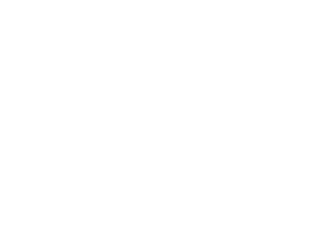
\includegraphics[width=\textwidth]{figures/theory/laminarFlow.pdf}
\caption{This shows the principal difference between laminar and turbulent flow.}
\label{fig:laminar_flow}
\end{figure}


\subsection{Stokes Drag and Stokes's law}
The drag force $F_D$ exerted by a fluid on a spherical particle for $Re << 1$ is found using the so called Stokes's law \cite{introfluid2}

\begin{equation}
F_D = 6\pi \mu R v
\end{equation}

where $v$ is the velocity of the sphere relative to the fluid, $\mu$ is the dynamic viscosity and $R$ is the radius of the sphere. The terminal velocity of the sphere is found by equating the gravitational force $F_G$ acting on the sphere with the drag force. $F_G$ is

\begin{equation}
F_G = \Delta \rho g\cdot \frac{4\pi R^3}{3}
\end{equation}

where $\Delta \rho$ is the difference in density and $g$ is the specific gravity. We find that the terminal velocity of a sinking (or floating) sphere is

\begin{equation}\label{eq:fallingSphere}
v_s = \frac{2}{9} \frac{\Delta \rho}{\mu} g R^2
\end{equation}

%\subsection{Shear}
%
%\subsection{P\'{e}clet Number}
%The p\'{}clet number describes the ratio of thermal noise to other stuff. I really don't know anything about the piclet number.


\section{Euler angles and coordinate system}
When describing rotating particles it is common to use the so-called Euler angles $(\phi, \theta, \psi)$. A formal definition is given by Diebel \cite{Euler} but for the purposes of this thesis we describe them as a transformation. We start with a stationary right-hand coordinate system $\{x,y,z\}$ with the $x$-axis along the length of the channel, the $z$-axis along the width of the channel, and the $y$-axis along depth. We define the Euler angles as the transformation from the channel coordinate system to the coordinate system attached to our particle $\{x',y',z'\}$. This transformation is performed in three steps by using an intermediate axis T.

\begin{itemize}
\item Rotate the $x$-$y$ plane $\phi$ radians about the $z$-axis. 
\item Denote the shifted $x$-axis $T$ and rotate the $z$-$y'$ plane $\theta$ radians around the $T$-axis
\item Denote the shifted $z$-axis $z$' and rotate the $x'$-$y'$ plane $\psi$ radians around the $z$' axis.
\end{itemize}

This procedure is illustrated in Figure \ref{fig:eulerangles} where each prime marks one additional step of rotation to the coordinate system. Figure \ref{fig:eulerparticle} shows the Euler angles for a triaxial particle from a point of view similar to that of the experiment where the $x$-$z$ plane is the field of view. Note that although $\psi$ has an impact on the particle dynamics, we cannot observe it in our experiment as the particles are too symmetric around that axis, as is shown in section \ref{sec:particle_improves}


\begin{figure}[H]
\centering
\begin{subfigure}[b]{0.45\textwidth}
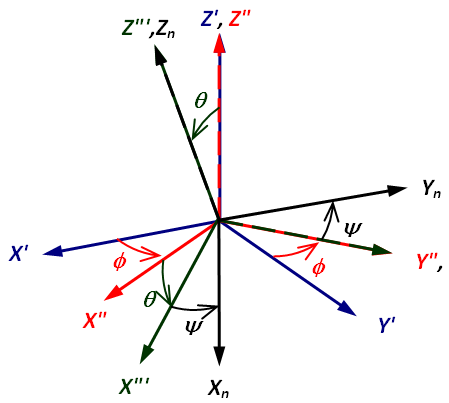
\includegraphics[width=0.9\textwidth]{figures/theory/eulerangles.png}
\caption{A general illustration of the Euler angles}
\label{fig:eulerangles}
\end{subfigure}
\begin{subfigure}[b]{0.45\textwidth}
\includegraphics[width=0.9\textwidth]{figures/theory/Euler3.pdf}
\caption{The Euler angles as used in our experiment}
\label{fig:eulerparticle}
\end{subfigure}
\caption{Figure (\subref{fig:eulerangles}): The Euler angles illustrated using a series of coordinate rotations. 
Figure (\subref{fig:eulerparticle}): The Euler angles illustrated using an ellipsoid. This alternate visualization shows the angles with a point of view similar to that of the camera in the experiment. }\label{fig:eulerplots}
\end{figure}


\begin{figure}[H]
\begin{center}
\includegraphics[width=0.5\textwidth]{figures/theory/defineN.pdf}
\end{center}
\caption{The unit vector $\mathbf{n}$ and its components $n_x$, $n_y$ and $n_z$. The vector $\mathbf{n}$ is a unit vector, $|\mathbf{n}| = 1$.}
\label{fig:nDef}
\end{figure}

The conversion from $(\phi, \theta, \psi)$ to the unit vector $\mathbf{n} = (n_x, n_y, n_z)$ is given by 

\begin{subequations}\label{eq:nzEq}
\begin{align}
n_x 	&= \sin(\theta)\cos(\psi), \\
n_y 	&= \sin(\theta)\sin(\psi),\\
n_z		&= \cos(\theta).
\end{align}
\end{subequations}

\noindent In particular $n_z$ and $\cos(\theta)$ are be used interchangeably.

\subsection{Triaxial particles}
A triaxial particle is an ellipsoidal particle that has a distinct radius around the $x$-axis, $y$-axis and $z$-axis. In other words it has distinct length, width and height. We refer to these lengths as $a_1, a_2, a_3$ with $a_1 > a_2 > a_3$.

%Triaxial particles have, as the name suggests, three axes which have distinct lengths. I will in this thesis refer to the lengths of these axes as  corresponding to their lengths along the $(x,y,z)$ axes when the rotation vector $\mathbf{E} = (0,0,0)$. 

When discussing triaxial particles that are close to being axisymmetric of the form $a_1 \gg a_2 \approx a_3$, it is convenient to introduce the particle asymmetry $\epsilon$ defined as

\begin{equation}\label{eq:epsilon}
\epsilon = \frac{a_2}{a_3} - 1,
\end{equation}

\noindent and the aspect ratio $\lambda$ given by

\begin{equation}\label{eq:lambda}
\lambda = \frac{a_1}{a_2}.
\end{equation}

These parameters are as used by among others Yarin \emph{et al.}~\cite{Yarin}.
% Where are we talking about this elsehwere?
%When trying to estimate the orientation of the particle from a projection in the x-z plane we will also be interested in the normalized projection of the particle onto the x-z plane. This will be referred to as $\mathbf{n} = (n_x, n_y, n_z)$

%We are interested in the orientation of the particle

%\begin{equation}
%n(t) = (n_x(t), n_y(t), n_z(t))^\intercal.
%\end{equation}



\section{Jeffery orbits}
\label{sec:jeffery}
The Jeffery orbits describe the orientational motion of an ellipsoidal particle in Stokes flow. The general equations of motion for any ellipsoid in shear flow were found by Jeffery\cite{Jeffery} who also solved these equations of motion for axisymmetric ($a_1 \ne a_2 = a_3$) ellipsoidal particles. Solutions for asymmetric particles were found numerically by Yarin \emph{et al.}~\cite{Yarin} who also rewrote the equations in a different but equivalent form. The equations of rotational motion for a triaxial particle in shear flow are in the form of Yarin \emph{et al.}

\begin{subequations}\label{eq:jeffrey}
\begin{align}
\frac{d\theta}{dt} 	&= (g_2 \sin \psi + g_3 \cos \psi ) \sin \theta, \\
\frac{d\phi}{dt} 	&= \tfrac{1}{2} + g_3\sin \psi - g_2 \cos \psi,\\
\frac{d\psi}{dt}	&= g_1 + (g_2\cos \psi - g_3\sin \psi) \cos \theta. \\
\end{align}
\end{subequations}

\noindent The functions  $g_i$ are defined as

\begin{subequations}
\begin{align}
g_1 &= \frac{a_2^2 - a_3^2}{2(a_2^2 + a_3^2)} 
		\left(-\tfrac{1}{2}(\cos^2 \theta + 1 )\sin 2\phi \sin 2\psi + \cos\theta \cos 2\phi \cos 2\psi \right), \\
g_2 &= \frac{a_3^2 - a_1^2}{2(a_1^2 + a_3^2)}
		\left( -\cos\theta \sin 2\phi \sin\psi  +  \cos 2\phi \cos\psi \right), \\
g_3 &= \frac{a_1^2 - a_2^2}{2(a_1^2 + a_2^2)}
		\left( \cos\theta \sin 2\phi \cos\psi + \cos 2\phi \sin\psi \right).
\end{align}
\end{subequations}

\noindent Here $(\phi, \theta, \psi)$ are the Euler angles seen in Figure \ref{fig:eulerangles}. 
%Note that Yarin uses $a_x, a_y, a_z$ in place of $a_1, a_2, a_3$.

Note that the eq. (\ref{eq:jeffrey}) uses the coordinate system from Yarin \emph{et al.}\cite{Yarin} which differ from the one used in this thesis, details are discussed in Johansson \cite{AntonThesis}. Numerical solutions for three different initial conditions for an asymmetric particle are shown in Figure \ref{fig:orbitparams}.

\begin{figure}[H]
\centering
\begin{subfigure}[b]{0.45\textwidth}
\includegraphics[width=\textwidth]{figures/theory/map.pdf}
\caption{A poincare map}\label{fig:orbitmap}
\end{subfigure}\hspace{1em}%
\begin{subfigure}[b]{0.5\textwidth}
\includegraphics[width=\textwidth]{figures/theory/orbit.pdf}
\caption{The time series for the components \\ of the unit vector.}\label{fig:orbitparams}
\end{subfigure}
\caption{A Poincare map and three different orbits for a simulated particle with $\lambda=7$ and $\epsilon=0.05$. The three orbits highlight the three different kinds of motion, the quasi-periodic sign changing orbit in blue, the quasi-periodic sign preserving orbit in red and the periodic orbit in green. We see that while $n_x$ and $n_y$ look qualitatively similar but differ in amplitude for the different orbits, $n_z$ shows three different types of behaviour}
\label{fig:orbittypes}
\end{figure}



Looking at Figure \ref{fig:orbitparams} we see that $n_x$ and $n_y$ are periodic, corresponding to periodic rotation around the $z$-axis. We refer to these rotations as flips. The period $\eta$ of $n_x$ and $n_y$ is for an axisymmetric particle \cite{Jeffery}

\begin{equation}\label{eq:flipRate}
\eta = 2\pi \left( \lambda + \frac{1}{\lambda} \right)\frac{1}{\kappa},
\end{equation}

\noindent where $\kappa$ is the shear rate. 

The time evolution of $\theta$ and $\psi$ for different initial conditions can be plotted in a Poincaré map, also known as a Surface-of-Section (S.O.S.)~\cite{poincare}. This plots the $\psi$ and $\theta$ coordinates each time $\phi = 0$. The successive points on the Poincaré map for each initial condition move and explore certain regions of the surface of section. This region is referred to as the \emph{orbit}. 

For a particle with an asymmetry $\epsilon$ in the range $\left[0.01-0.05\right]$ there are three classes of orbits, depending on the initial condition $\theta_0$.

\begin{enumerate}
\item \textbf{Periodic}: $\left|\theta_0\right| \approx 1$ in which there is little variation and the particle is largely periodic with fluctuations too small to measure.
\item \textbf{Quasi-periodic sign preserving}: For $\left|\theta_0\right|> \theta_b$ the amplitude of $\cos(\theta)$ changes noticeably but does not change sign. Here $\theta_b$ is a breaking point that changes for different $\epsilon$.
\item \textbf{Quasi-periodic sign changing}: For small $\left|\theta_0\right| < \theta_b$ the amplitude of $\cos(\theta)$ changes noticeably and changes sign. 
\end{enumerate}

Simulations of these three different types of orbits for a particle with $\lambda=7$ and $\epsilon=0.05$ are illustrated in Figure \ref{fig:orbittypes}. Figure \ref{fig:orbittypes} shows the orbits on the S.O.S. and Figure \ref{fig:orbitparams} shows the components of $\mathbf{n}$ as a function of time. We can see that while $n_x$ and $n_y$ are periodic, albeit with different amplitudes, the  behaviour of $n_z$ is significantly different for the different orbits. The $n_z \approx 1$  orbit shown in green is constant on the S.O.S and is simply periodic over time. The sign preserving quasi-periodic orbit in red is bent on the S.O.S. We can see in the time series that it is doubly periodic as it peaks with a fixed period but the amplitude of the peaks vary periodically themselves. The sign changing quasi-periodic orbit in blue also peaks periodically with varying peak amplitude but these also change sign, again with a fixed period.


For larger asymmetries $\epsilon > 0.05$ there are chaotic orbits that explore a larger region of the S.O.S. The simulations used do not have long enough time evolutions for the chaotic orbits to fill the regions in the way that quasi-periodic or periodic orbits fill the one dimensional regions that define their orbits. This results in the chaotic orbits appearing as a 'sea' of dots instead of filled lines. Chaotic orbits can been seen around the quasi-periodic sign changing orbits in Figure \ref{fig:orbitmap4}.

\begin{figure}[H]
\centering
\begin{subfigure}[3a]{0.40\textwidth}
\includegraphics[width=\textwidth]{figures/theory/7-1-1.pdf}
\caption{Poincare map for $\lambda = 7, \epsilon = 0$.}\label{fig:orbitmap1}
\end{subfigure}\hspace{1em}%
\begin{subfigure}[3b]{0.40\textwidth}
\includegraphics[width=\textwidth]{figures/theory/7-1o01-1.pdf}
\caption{Poincare map for $\lambda = 7, \epsilon = 0.01$.}\label{fig:orbitmap2}
\end{subfigure} \\
\begin{subfigure}[3a]{0.40\textwidth}
\includegraphics[width=\textwidth]{figures/theory/7-1o05-1.pdf}
\caption{Poincare map for $\lambda = 7, \epsilon = 0.05$.}\label{fig:orbitmap3}
\end{subfigure}\hspace{1em}%
	\begin{subfigure}[3b]{0.40\textwidth}
\includegraphics[width=\textwidth]{figures/theory/7-1o25-1.pdf}
\caption{Poincare map for $\lambda = 7, \epsilon = 0.25$.}\label{fig:orbitmap4}
\end{subfigure} 
\caption{Four Poincare maps for different $\epsilon$. Already at $\epsilon = 0.01$ there are noticeably quasi-periodic 
orbits around the centre at $\cos(\theta) \approx \psi \approx 0$ but it is also a significantly larger region for $\epsilon = 0.05$. For $\epsilon = 0.25$ we can see chaotic orbits surrounding the circular orbits in the centre that appear as a 'sea' of dots.} %q Note that some wavelike pattern can appear to exist in the figure \ref{fig:orbitmap2} and  \ref{fig:orbitmap2}, this is caused by aliasing/compression issues with printing several curved lines close together.}\label{fig:orbitmaps}
\end{figure}

\subsection{Winding number} \label{sec:winding}
The quasi-periodic orbits are also referred to as doubly-periodic~\cite{Yarin}. It is called doubly-periodic to emphasize the fact that the amplitude of the short period $\theta_2$ also varies periodically with period $\theta_1$. The ratio between the two periods is referred to as the winding number $\omega$ referring to the winding around a unit torus. The shorter period $\theta_2$ corresponds to rotations around the small cross section and the longer period $\theta_1$ corresponds to rotations around the large circumference of the torus. The winding number is defined as \cite{introchaos}

\begin{equation}
\omega_{def}  = \lim\limits_{n \rightarrow \infty} \frac{f^n(\xi) - \xi_0}{n}.
\end{equation}

where $\xi$ is the angle around the large circumference of the torus and $f^n(\xi)$ is the shift caused in $n$ rotations around the smaller axis. 
Applying this to our double-periodic orbits $\xi$ would be the angle with period $\theta_1$ and $n$ the number of flips with period $\theta_2$. 
Since we cannot measure $\xi$ I consider it more comprehensible to consider the inverse winding number: The number of flips necessary to 
complete one period of $\xi$. This can be measured as is shown in Figure \ref{fig:windingDef}. If we measure over several $\theta_1$ peaks the average winding number approximates the real one. We refer to the this inverse winding number as $\omega$ and it is given by

\begin{equation}\label{eq:winding}
\omega = \frac{\theta_1}{\theta_2}.
\end{equation}

\noindent The winding number of the quasi-periodic sign preserving orbit from Figure \ref{fig:orbittypes} and the way we approximate $\theta_1$ (and thereby $\omega$) is illustrated in Figure \ref{fig:windingDef}.

\begin{figure}[H]
\begin{center}
\includegraphics[width=0.7\textwidth]{figures/theory/WindingNrFixed2.pdf}
\end{center}
\caption{The quasi-periodic sign preserving orbit from Figure \ref{fig:orbitparams} over a longer time, highlighting the short period $\theta_2$ which is simply the period of $\phi$ and the longer period $\theta_1$. We find the inverse winding number as the ratio between the longer and shorter periods.}
\label{fig:windingDef}
\end{figure}

%This can also be thought of as the number of intersections on the surface of section before coming back to the initial condition, divided by the number of laps. A lap for a circular orbit is a rotation around the center whereas for a flat orbit it is moving along length of the orbit. asdasd, see figure MAKE A FIGURE. 
The winding number is the same for any point along a quasi-periodic orbit on a Poincaré map but it is different for different orbits as well as for different asymmetries. The winding numbers for orbits along $\psi=0$ for $\epsilon=\{0.01, 0.05, 0.10\}$ can be seen in Figure \ref{fig:windingdifferent}. The difference in winding number between the different $\epsilon$ for the sign changing orbits are almost a factor 2. This means that if we can measure the winding number for a sign changing orbit it allows us to approximate the asymmetry of the particle even though the variation in $n_z$ are identical. Without looking at the winding number we cannot determine if a particle with an orbit close to $n_z = 0$ and small variations in amplitude is close to symmetric or not.
 
\begin{figure}[H]
\begin{center}
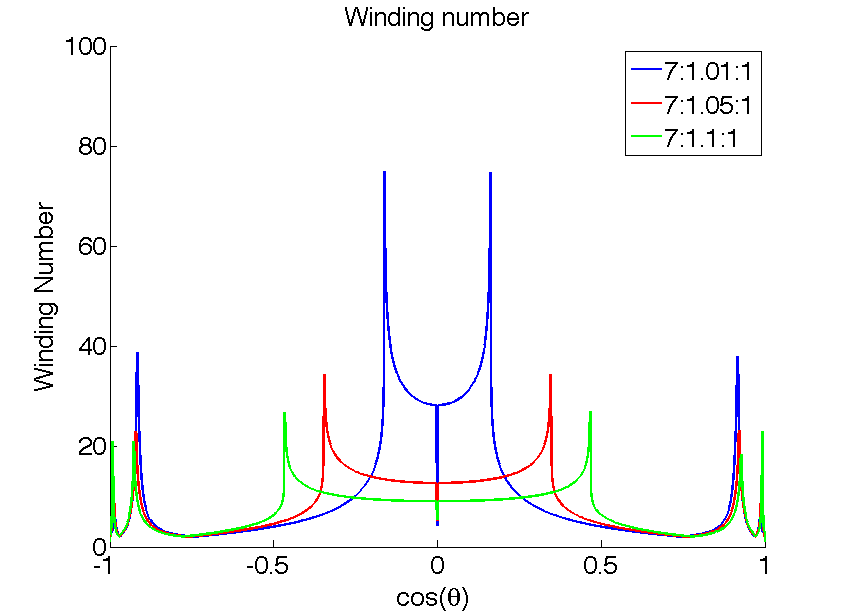
\includegraphics[width=0.7\textwidth]{figures/theory/WindingTrend.png}
\end{center}
\caption{The winding number for $\psi_0 = 0$ and $\lambda = 7$ as a function of $\cos(\theta_0)$ for three different asymmetries, $\epsilon = 0.01$, $\epsilon = 0.05$ and $\epsilon = 0.10$. The sharp edge that occurs at different points for the different asymmetries, but centred around zero, is where the sign changing orbits end and sign preserving orbits begin, denoted by $\theta_b$. We see that a lower asymmetry leads to a sharper difference between the sign changing and the sign preserving orbits and that higher asymmetry in general leads to lower winding numbers on average.}
\label{fig:windingdifferent}
\end{figure}


\chapter{Method}
\part{Improvements of experimental setup}


To measure Jeffery orbits we need to have an experimental setup with which to measure. The one used in this thesis is an iteration of the one used by Einarsson \emph{et al.}~\cite{JonasExperiment}, Johansson \cite{AntonThesis}, and Mishra \emph{et al.}~\cite{Mishra}. In this chapter we describe the setup and why it is designed the way it is. We also discuss the improvements over previous iterations, as well as new problems that have arisen from the changes made. In particular we describe a tracking algorithm that was implemented to make gathering data easier.
\section{Experimental setup}
\label{sec:exp_setup}
The orientational motion of $\mu$m sized particles suspended in a liquid was investigated by pumping the liquid through a microfluidic channel using a syringe pump. The channel is placed on a moveable stage on top of a microscope. A particle is tracked by moving the stage to match the center of mass velocity of the particle in the channel and thus keep the particle stationary in the field of view of the microscope. Connected to the microscope is a CCD camera recording the images and these movies are saved on a computer. 

When the tracked particle gets within \unit[1]{cm} of the inlets on the channel the flow is reversed. In order to reduce sudden impact of the pressure difference the reversals are incremental. At the start of a reversal the infusion/withdrawal rate is reduced by 50\% for 10 seconds, then stopped completely for 10 seconds. After this the flow is reverted at 50\% of the normal flow rate for another 10 seconds before resuming at full speed. 

We refer to the data of a particle along one length of the channel a \textbf{stretch} and a series of stretches for a single particle a \textbf{measurement}. A sketch of the experimental setup can be seen in figure \ref{fig:setupsketch}, and a photograph of the actual setup in figure \ref{fig:setuppicture}. 

Between measurements, optical tweezers constructed by A. Laas were used to change the orientation of the particle. For details on optical tweezers function see the introductory guide from Stanford \cite{OpticalTweezer} or Laas thesis \cite{alexanderThesis}. 


\begin{figure}[H]
\centering
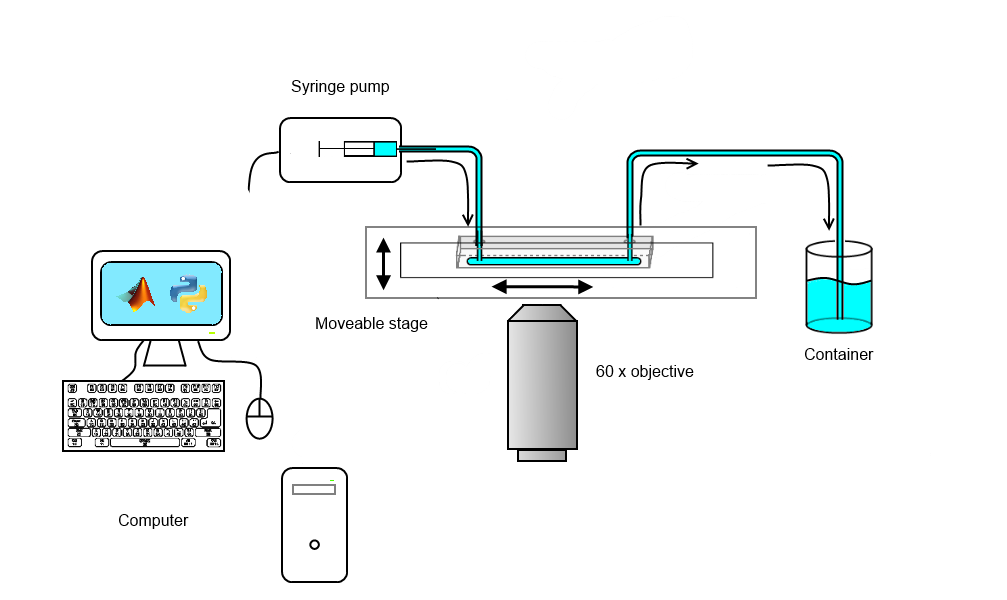
\includegraphics[width=0.8\textwidth]{figures/method/setupsketch.png}
\caption{Sketch of the set up. The computer controlled stage moves over the microscope. The pump reverses when the tracked particle gets close to the inlets of the channel.}\label{fig:setupsketch}
\end{figure}

% Have both this zoomed out and the zoomed in view I think
\begin{figure}[H]
\centering
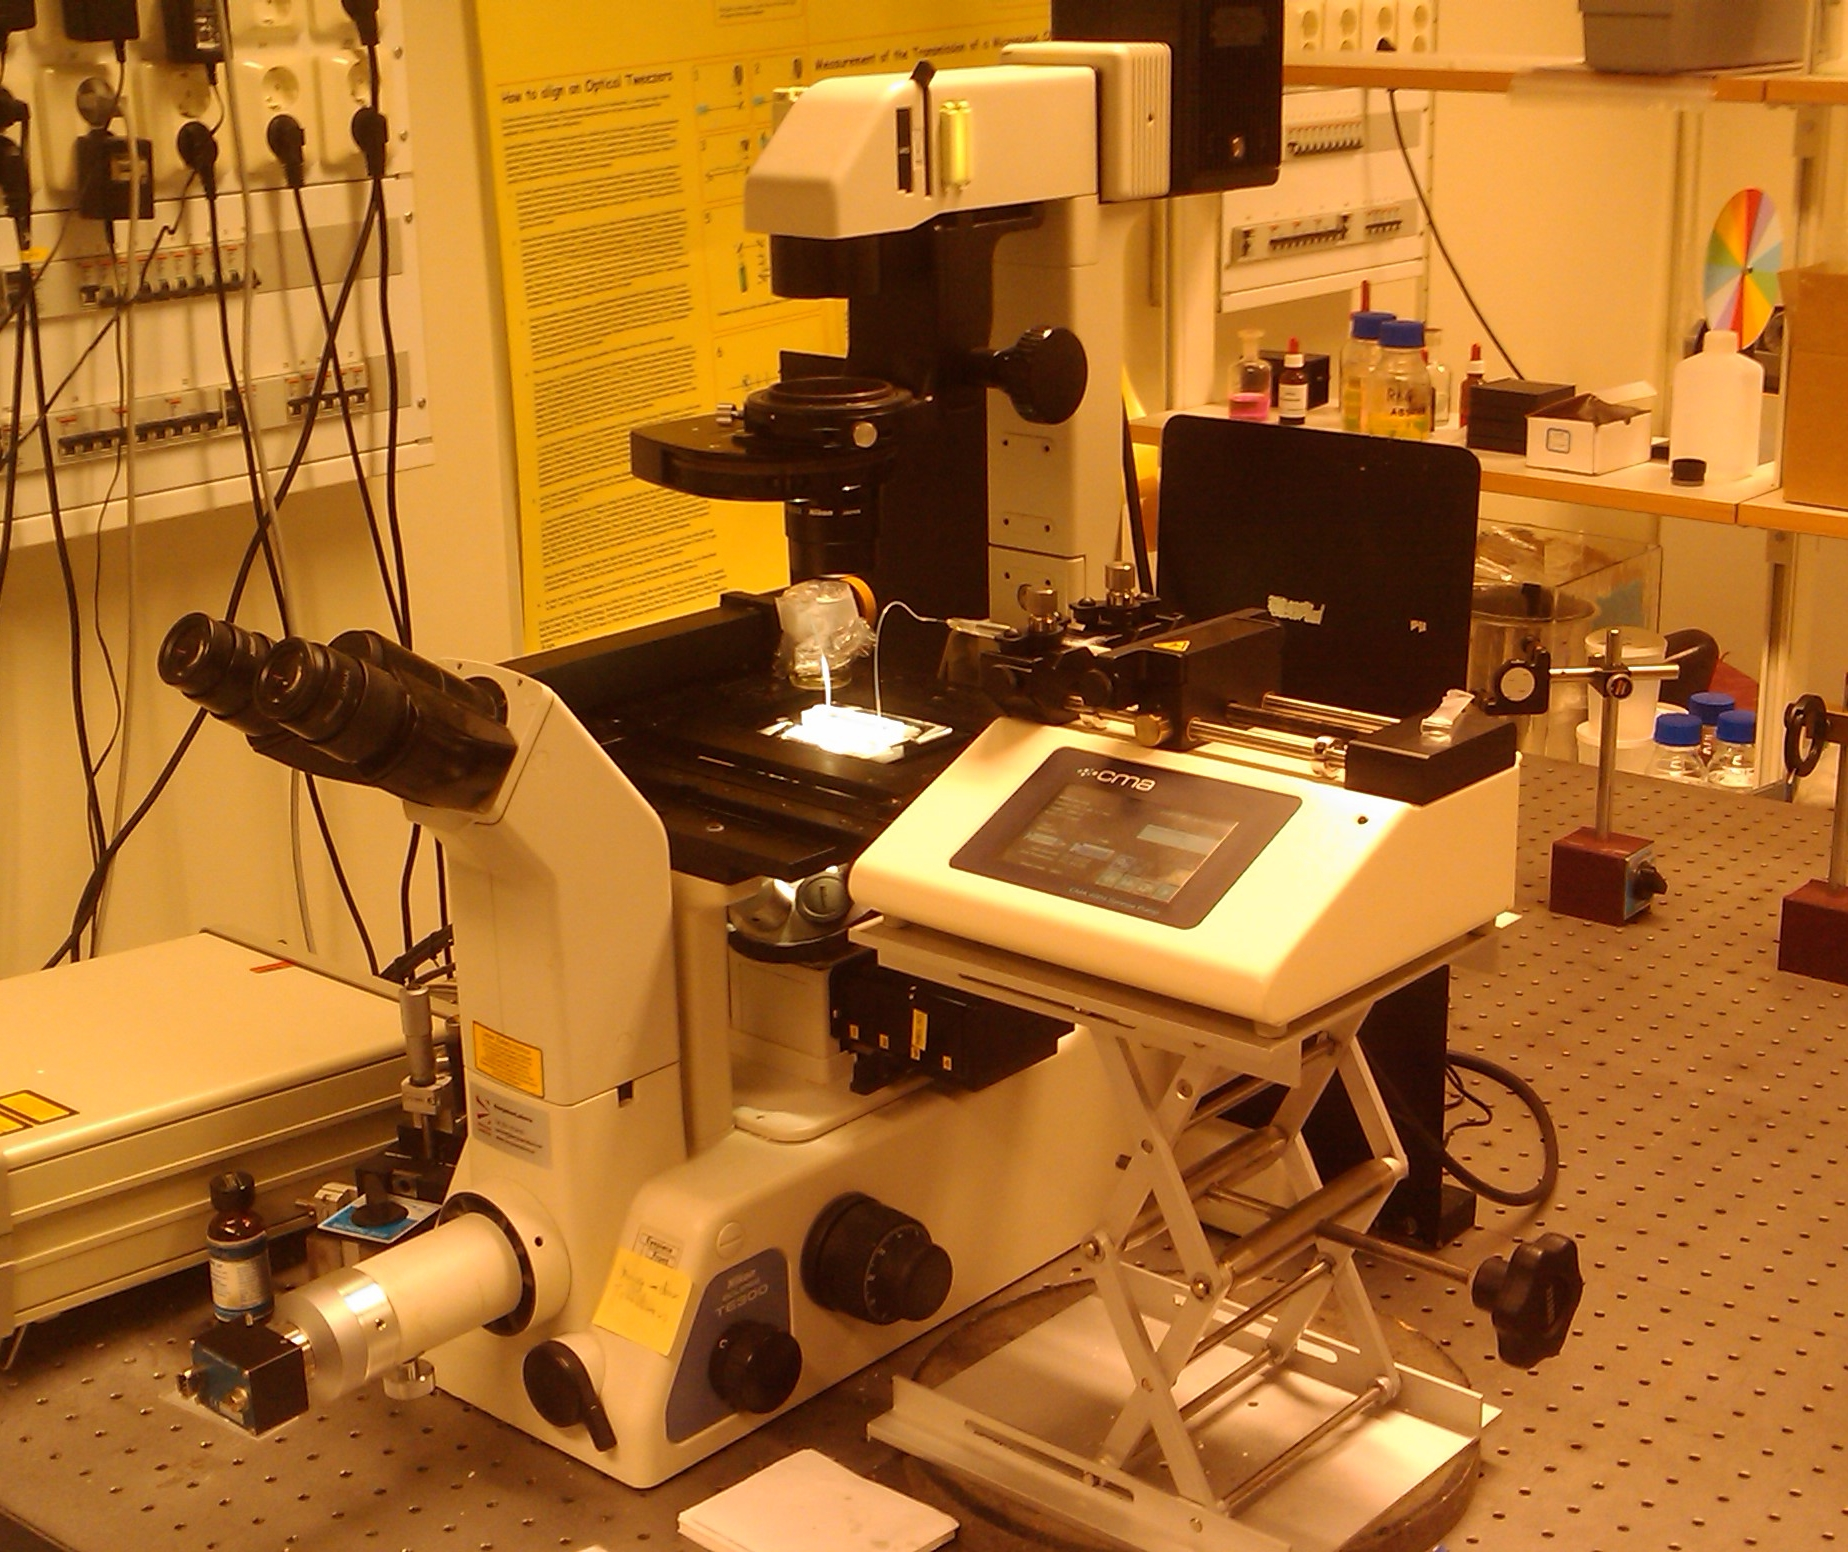
\includegraphics[width=0.8\textwidth]{figures/method/ExperimentalOverview.jpg}
\caption{Overview of the set up. The microscope to the left and the syringe pump to the right. In the center is the channel and the outlet container is seen behind it. The CCD camera is mounted on the left side of the microscope and cannot be seen in this picture.}\label{fig:setuppicture}
\end{figure}


The microfluidic channel is \unit[40]{mm} long, \unit[2.5]{mm} wide and approximately \unit[150]{$\mu$m} deep. The channel is made from Polydimethylsiloxane (PDMS) and plasma bonded to a microscope slide. A more detailed description of the process can be found from the Center for Computer Integrated Systems for Microscopy and Manipulation~\cite{PDMS}. This material and procedure is chosen so that a channel that gets filled with dirt or breaks can cheaply and easily be replaced. PDMS is also non-reactive and highly transparent. A sketch of the channel can be seen in figure \ref{fig:channelsketch}, and a photograph of an actual channel in figure \ref{fig:channelpicture}. 

\begin{figure}[H]
\centering
\begin{subfigure}[b]{0.45\textwidth}
\includegraphics[width=0.9\textwidth]{figures/method/channelDetail.pdf}
\caption{Sketch of the channel}\label{fig:channelsketch}
\end{subfigure}
\begin{subfigure}[b]{0.45\textwidth}
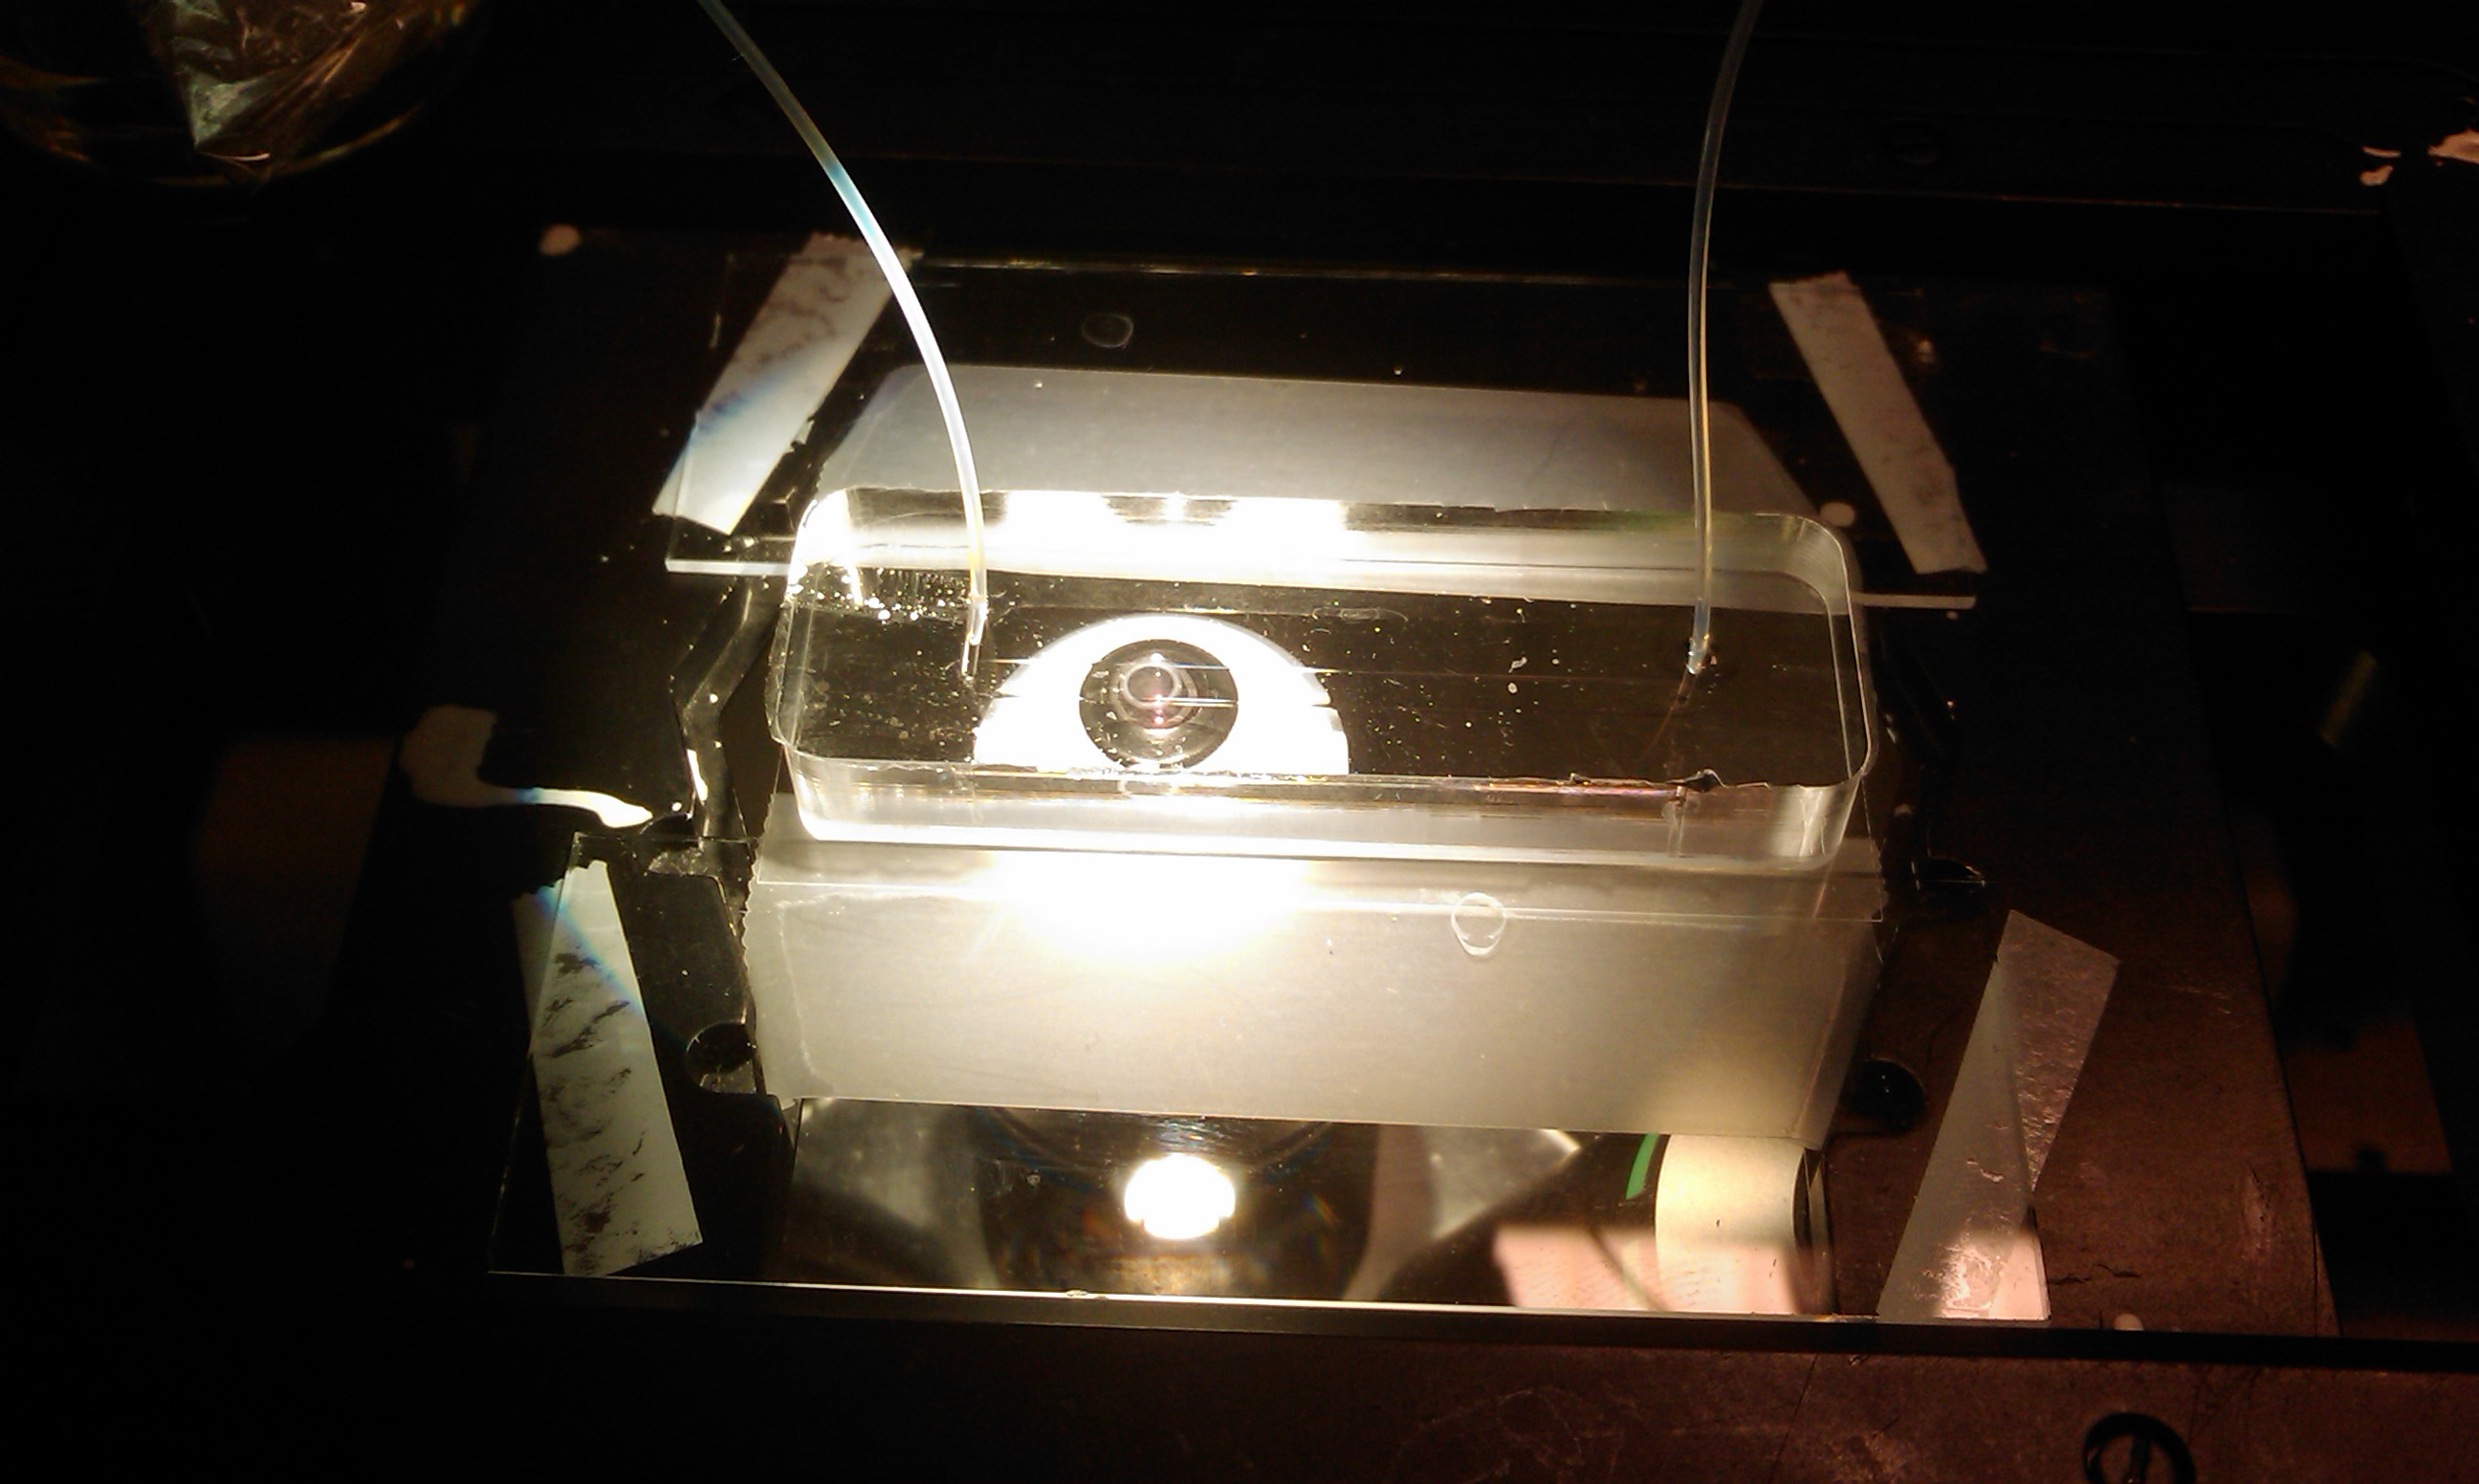
\includegraphics[width=0.9\textwidth]{figures/method/ChannelZoomed.jpg}
\caption{Picture of the channel}\label{fig:channelpicture}
\end{subfigure}
\caption{A sketch of the channel as well as a picture of the channel as it is set up during a measurement. The channel is only \unit[150]{$\mu$m} deep, but the PDMS surrounding it is around 15 mm to try and prevent the channel from expanding and contracting too much.}
\label{fig:channel}
\end{figure}

% rewrite
In order to find the maximum flow speed of the channel we need to know the flow profile. Using the software employed by Johansson \cite{AntonThesis} we obtain the flow profile that can be seen in figure \ref{fig:flowprofile}. Integrating 
the flow profile over the entire surface will give us an effective flow area, essentially how large the channel 'actually' is. 
Using the flow profile from figure \ref{fig:flowprofile} we find that the effective flow area is $\unit[0.14]{mm^2}$. With a pump rate of \unit[7.5]{$\mu$l/minute} we get a maximum velocity of \unit[0.90]{mm/s} for the liquid.

% PIcture of the channel meassurements here 


% Picture of channel flow profile
\begin{figure}[H]
\begin{center}
\includegraphics[width=0.7\textwidth]{figures/method/flowprofile.pdf}
\end{center}
\caption{The theoretical estimation of the flow profile. Image generated with software from Johansson \cite{AntonThesis}, used with permission.}
\label{fig:flowprofile}
\end{figure}

\noindent We need to confirm that the flow is has no inertial effects. We can calculate the maximum Reynolds number using eq \ref{eq:reynolds}, the \unit[3]{$\mu$m} length rods, and our maximum flow speed.

\begin{equation}
\operatorname{Re_p} = \frac{U L \rho}{\mu} 
\leq \frac{9.0\cdot 10^{-4} \cdot 3 \cdot 10^{-3} 2.5 }{24 \cdot 10^{-3}} 
\approx	 	2.78  \cdot 10^{-6} \ll 1
\end{equation}

This should satisfy the conditions of validity for the Jeffrey equations. 

To track the particles the channel is put in a moveable stage on a confocal microscope. The entire setup can be seen in figure \ref{fig:setuppicture}



\subsection{List of equipment}
 The equipment used during the experiment is as follows
\begin{itemize}
\item Leica DFC350 FX digital camera 
\item Nikon Eclipse TE 300 microscope
\item Nikon 60x water immersion objective
\item Märzhäuser Wetzlar 'LStep-eco' step engine
\item CMA 4004 syringe pump
\item Ytterbium fiber laser  % What laser?
\end{itemize}

%
%\subsection{Density matching}
%\begin{equation}
%\rho_{a} = 	\frac {m_{a}}{V_{a}} =
%				\frac{V_{b}\rho_{b} + V_{mix}\rho_{mix}}{V_b + V_{mix}} 
%\end{equation}
%So if we want to find $V_{mix}$ we get
%\begin{equation}
%V_{mix} = \frac{ V_{b}(\rho_{b} - \rho_{a})}{\rho_{a} - \rho_{mix}} 
%\end{equation}
%
	
\section{Problems and improvements}
As previously mentioned this thesis is a continuation of work done by Mehlig, Einarsson and Mishra et al \cite{AntonThesis, JonasExperiment}. Their results were promising but there were a number of key limitations and problem that we want to solve to improve the results and the ease of getting results. Roughly they are
\begin{enumerate}
	\item The particles
	\begin{itemize}
		\item Very few particles are symmetric, most are visibly bent or uneven, see figure \ref{fig:oldparticles}
		\item Few particles have a low enough aspect to be useful.
		\item Have greatly varying and difficult to measure width meaning the aspect ratio cannot be estimated well
		\item Cannot be trapped with an optical tweezer due to low transmittance
	\end{itemize}
	\item The PDMS in the channel is very jagged which causes a great deal 
			of noise unless the focus is in a very narrow band
	\item Manual tracking of particles is time consuming and mentally draining.
	\item Bubbles are difficult to avoid when setting up the experiment
\end{enumerate}


\subsection{Particles and channel}
\label{sec:particle_improves}
\begin{figure}[H]
\centering
\begin{subfigure}[b]{0.45\textwidth}
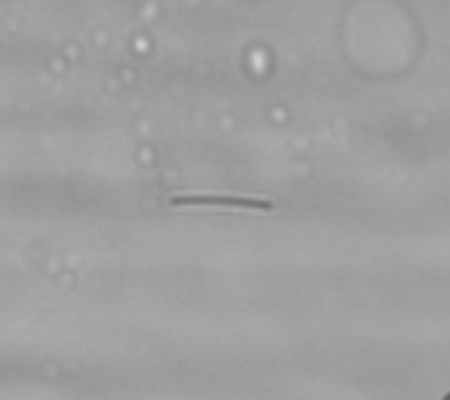
\includegraphics[width=0.9\textwidth]{figures/improvements/oldparticle2.png}
\caption{Particle 13 from July 2012}
\end{subfigure}
\begin{subfigure}[b]{0.45\textwidth}
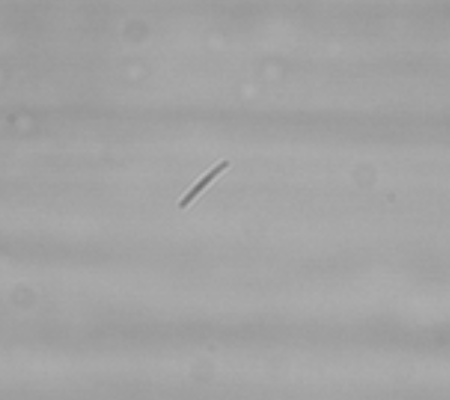
\includegraphics[width=0.9\textwidth]{figures/improvements/oldparticle3.png}
\caption{Particle 22 from July 2012}
\end{subfigure}
\caption{Two fairly typical particles from the previous setup. Note that these are still selected from the total pool of particles for being relatively symmetric and yet are noticeably bent.}
\label{fig:oldparticles}
\end{figure}



The polymer particles were replaced with glass particles from Nippon Glass, Japan \cite{Particles}. The new particles are made 
from LCD spacing rods that are broken into pieces. This means that they are essentially broken cylinders with very 
homogeneous widths but quite disparate lengths. Two different batches of particles have been used, one with a $3\mu m$ diameter and one batch with $5 \mu m$ diameter. All the measurements presented in the results section are from the $3 \mu m$ width particles. 

The symmetries of the particles were investigated with the help from Stefan Gustafsson by taking images with an 
ESEM (Environmental Scanning Electron Microscope) shown in figure \ref{fig:particlepictures}. We see that the 
particles are uniformly smooth along the sides but have varyingly jagged edges causing different degrees of asymmetry. 

In particular figure \ref{fig:roundparticle} shows a top down view of a particle clearly showing a very circular shape 
with no discernible asymmetry whereas figure \ref{fig:particlepictures} show the jagged edge of several particles. 


\begin{figure}[H]
\centering
\begin{subfigure}[3a]{0.40\textwidth}
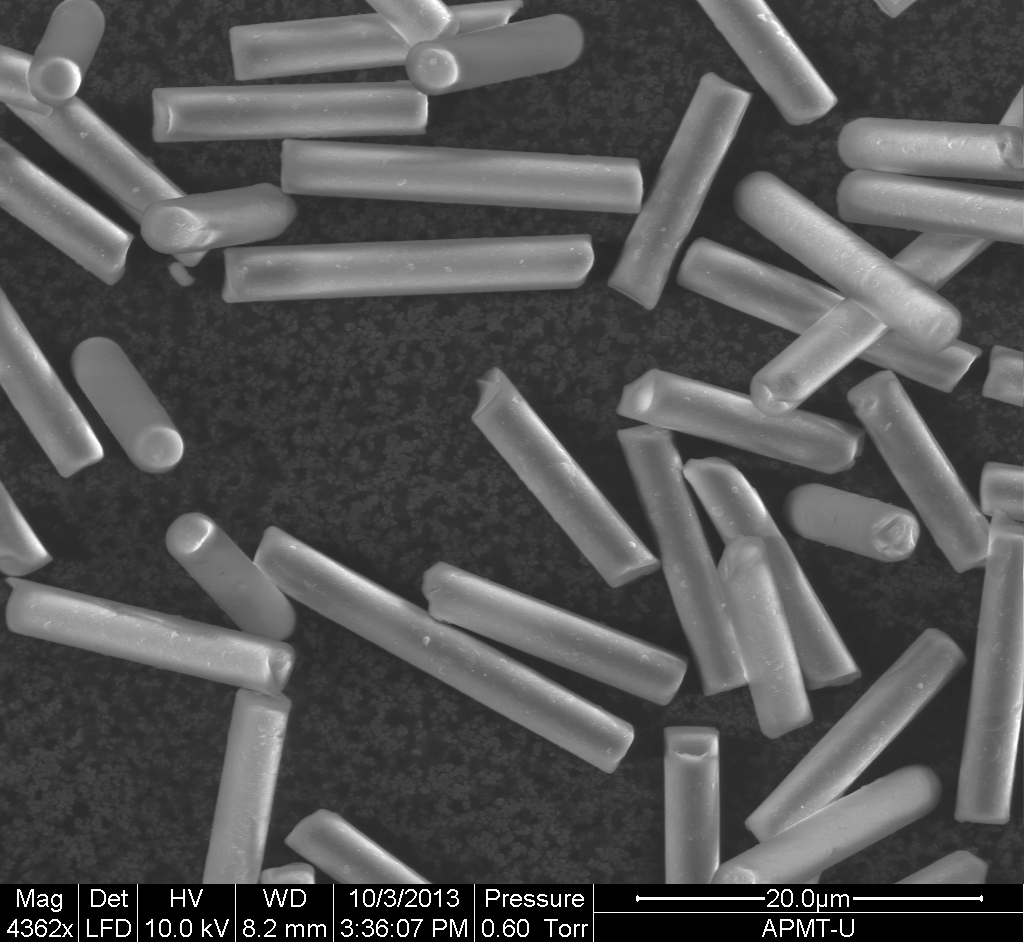
\includegraphics[width=\textwidth]{figures/method/semizoomed.png}
\caption{A detailed view \\ of a number of particles.}
\end{subfigure}\hspace{1em}%
\begin{subfigure}[3b]{0.40\textwidth}
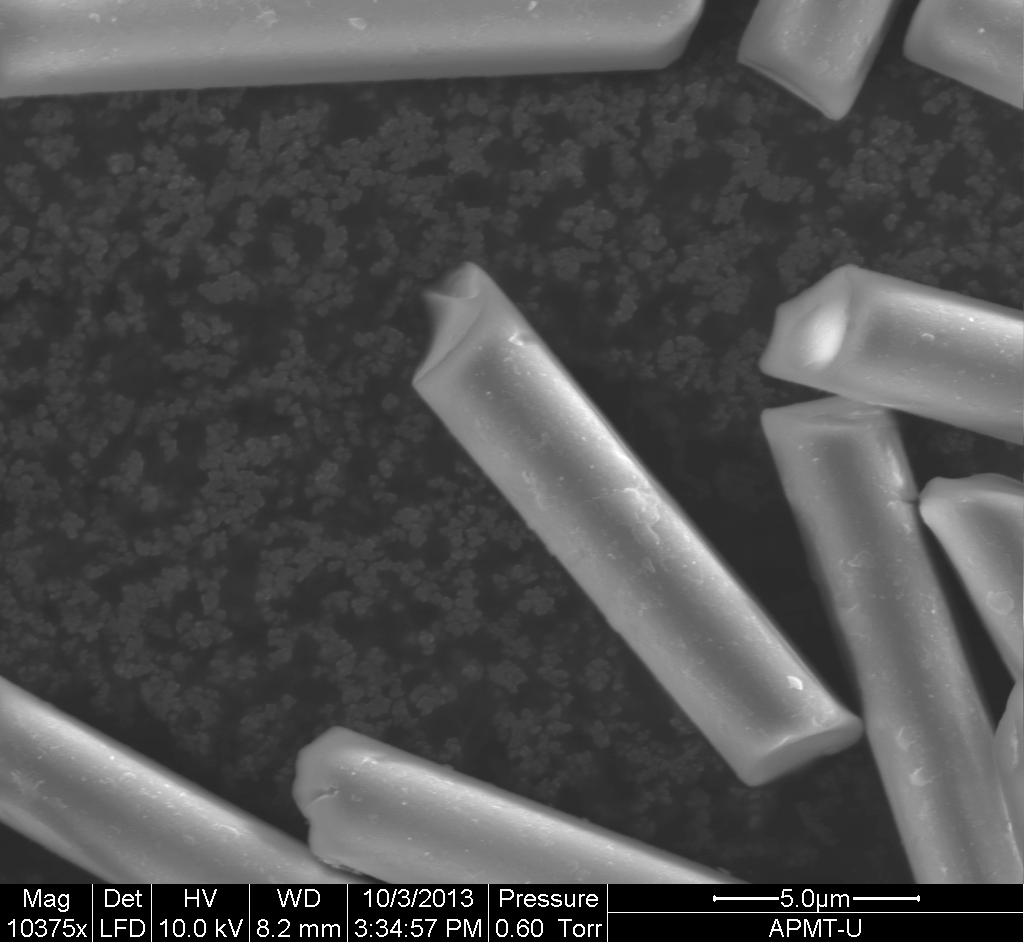
\includegraphics[width=\textwidth]{figures/method/zoomedbroken.png}
\caption{The jagged edge of a particle \\ in detail.}
\end{subfigure}
\caption{Pictures of the glass particles that were used. Their width is highly uniform and there is a noticeable variance is asymmetry. Some particles show very clearly jagged edges while other appear very smooth. This suggests that they should have quite different $\epsilon$ and then exhibit quite different behaviour.}
\label{fig:particlepictures}
\end{figure}
 
\begin{figure}[H]
\centering
\begin{subfigure}[3a]{0.40\textwidth}
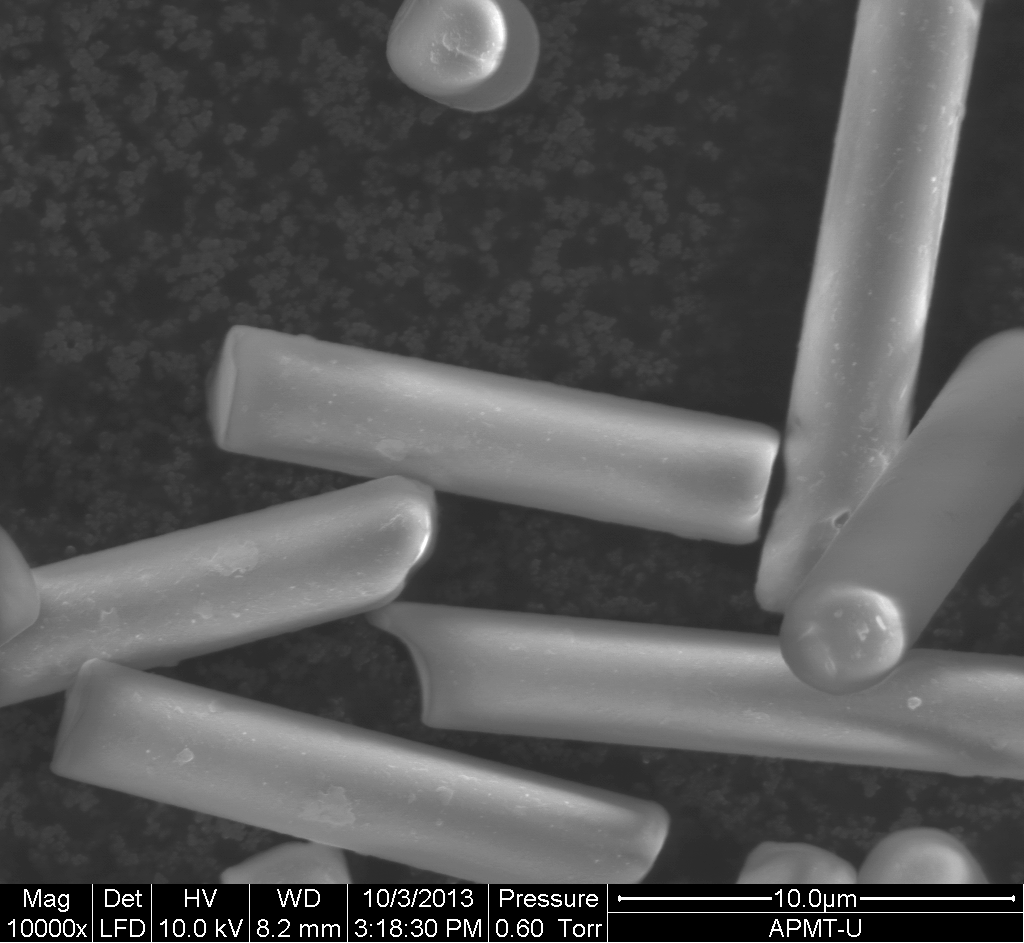
\includegraphics[width=\textwidth]{figures/method/symmetric.png}
\caption{What appears to be a highly \\ symmetric particle.}\label{fig:symmetricparticle}
\end{subfigure}\hspace{1em}%
\begin{subfigure}[3b]{0.40\textwidth}
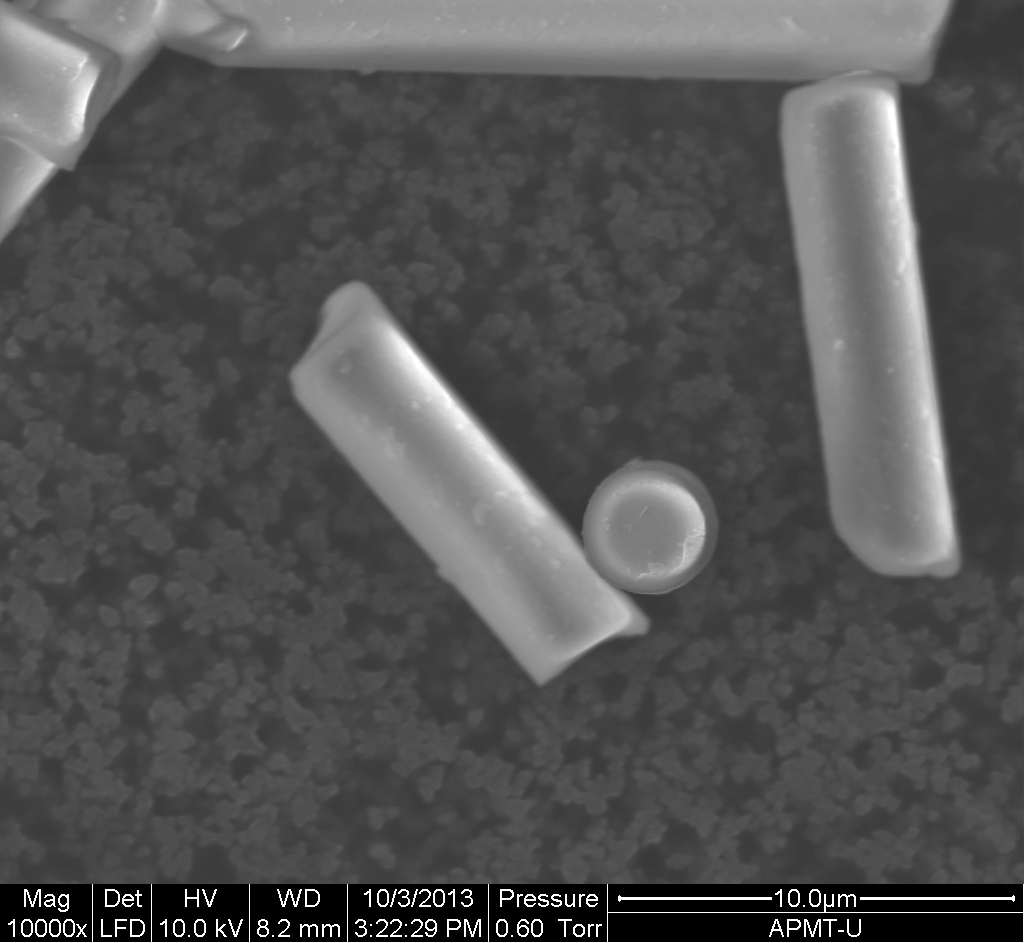
\includegraphics[width=\textwidth]{figures/method/round.png}
\caption{A top down view of a particle.}\label{fig:roundparticle}
\end{subfigure}
\caption{Pictures highlighting the roundness of the particles as well as the apparent symmetry of some particles. It should be noted that although there are no apparent rough edges there was no way to rotate a sample so there might very well be asymmetries on the side of the particle that we cannot see.}
\label{fig:particlepictures2}
\end{figure}

Figure \ref{fig:roundparticle} and \ref{fig:symmetricparticle} are the same as can be seen in \cite{alexanderThesis} figure 5.2(c) and 5.2(b) respectively. 

While these particles seemingly satisfy the symmetry conditions they are made of glass with a density of approximately 
\unit[2.57]{g/cm$^3$} at \unit[20]{C$^\circ$}. This is significantly higher than that of water with a density of 
\unit[1]{g/cm$^3$} at \unit[20]{C$^\circ$} and glycerol with a density of \unit[1.5]{g/cm$^3$}. Thus to correct for the 
density and limit sinking or floating the water soluble Sodium metatungstate which at \unit[20]{C$^\circ$} has maximum 
density of \unit[2.94]{g/cm$^3$} is added to the liquid. To increase the viscosity of the liquid around 8\% glycerol is added and the liquid 
was measured using a MCR 302 rheometer to have a dynamic viscosity of \unit[$24\cdot 10^{-3}$]{Pa s}.


A problem in finding and tracking a particle was that the surface of the PDMS was very uneven and sharp ridges along the length of the channel appear like in figure \ref{fig:unpolished} unless the focus was in a relatively narrow depth of the channel. 
 
 \begin{figure}[H]
 \centering
 \begin{subfigure}[3a]{0.40\textwidth}
 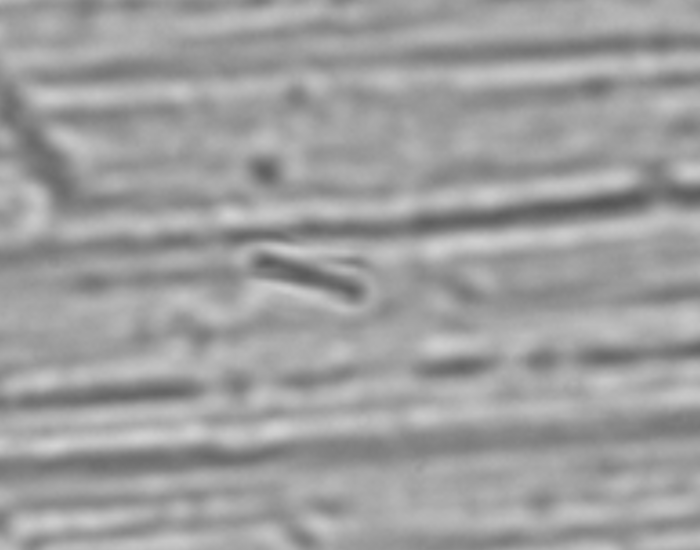
\includegraphics[width=\textwidth]{figures/improvements/unpolished.png}
 \caption{An unusually severe case of the PDMS edges creating noise.}\label{fig:unpolished}
 \end{subfigure}\hspace{1em}%
 \begin{subfigure}[3b]{0.40\textwidth}
 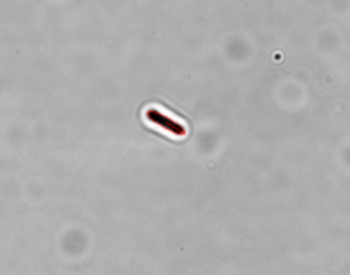
\includegraphics[width=\textwidth]{figures/improvements/polished.png}
 \caption{After being polished there is no trace of such ridges.}\label{fig:polished}
 \end{subfigure}
 \caption{Pictures highlighting the roundness of the particles as well as the apparent symmetry of some particles. It should be noted that although there are no apparent rough edges there was no way to rotate a sample so there might very well be asymmetries on the side of the particle that we cannot see.}
 \label{fig:polisheffect}
 \end{figure}
 

This was fixed by polishing the copper mold in which the PDMS channels are formed with a silicate abbrasive (Autosol) and emery cloth. This reduces all visible scratches from the mold and thus from the PDMS and the result can be seen in figure \ref{fig:polished}.



\section{Automated tracking}
%GENERAL LAYOUT
%
%Why we want tracking 
%
%The differences between tracking and tracking
%
%The methods used
%
%The limitations
%
%1) Why we want tracking

One of the most time consuming aspects as well as mentally draining is manually tracking a particle. Depending on the flow rate and the number of stretches and runs desired for a particle it can take several hours. Thus one of the primary targets for improvement as discussed by Johansson \cite{AntonThesis} was to try and make the camera tracking automatic. This would enable faster measurements as well as more measurements since it would reduce fatigue. 

Such a tracking was implemented using Python and the external packages \texttt{OPENCV}, \texttt{NumPy}, \texttt{SciPy}, \texttt{ImageMagick} and \texttt{ctypes}. The goal of the tracking is relatively similar to the tracking described in \ref{sec:particleTracking} and more in detail in Johansson \cite{AntonThesis} however there are a few very important differences that produce unique problems. 

\subsection{Aquiring the image}
The first step in this is to acquire the image from the micrscope in order to identify (and track) the particle. However the Leica DFC350 FX camera only works with the proprietary Leica software which means there is no easy way to get this image straight from the camera in real time. This meant we were forced to use the \texttt{ImageGrabber} package in \texttt{Python} and then isolate the camera image from the screen. This quite easy to do but takes ca 50ms per frame which would be unnecessary for an open source camera software. 

\subsection{Removing noise}
The first step is to reduce the static noise from the movie caused by dirt, scratches and other defects in the microscope and on the camera lens as can be seen in figure \ref{fig:origFrame}. As the noise is static and everything else changes this is a simple matter of computing an average frame

\begin{equation}\label{eq:averageFrame}
\bar{F} = \frac{\sum\limits_{n=1}^{N} F }{N}
\end{equation}

an example of such an average frame can be seen in figure \ref{fig:averageFrame}. This is then removed from the camera frame and the result can be seen in figure \ref{fig:fixedFrame}. After this we apply a smoothing function and Canny edge detection \cite{Canny} and then use the resulting edge. 

\subsection{Contour detection and selection}

Once an edge image has been generated, we use the OpenCV command, \texttt{Contours} which returns a list of every contiguous group of edge pixels. If we have chosen the threshold values to the edge detection correctly, this should include the particle or a good approximation of it. 

In order to find the correct contour  a few techniques are used.

First contours whose total size is less than some minimum value, $ n_{min}$ or larger than some maximum value $n_{max}$ are ignored. Then the position $P_i$ of each contour $C_i={p_1,p_2...p_n}$ is calculated as the average pixel position

\[
P_i = \sum_{j}^n p_j/n
\]
This position is compared to the expected position of the particle , which the very first frame is the middle position and thereafter is assumed to have constant speed. 

Finally a 'thinness value' is calculated according to eq \ref{eq:thinness}

\begin{equation}\label{eq:thinness}
w_{thin}\left(\frac{ n}{d_{max}^2}\right)^2
\end{equation}. 
where $w_{thin}$ is a weighting constant, $n$ is the number of pixels in the contour and $d_{max}$ is the longest distance between two pixels in the contour.
% Mostwhere I am not really sure I should do this now that I have so few particles, but I do it none the less!

\subsection{Adjusting the Camera velocity}
Once detected twice the particle will have some velocity relative to the camera $v_{rel}$ and a position $\mathbb{P}$. 
If the velocity is larger than some threshold $v_{thresh}$ or the position is outside a center square in the image, $\mathbb{P} \not \in \mathbf{B}$ we want to adjust the velocity of the step engine. 

We then simply do a straight correction but with a damping factor $\zeta$ to prevent a feedback loop. So our resulting velocity change $V_c$ is 

\begin{equation}
V_c = v_{rel}\cdot \zeta
\end{equation}

\subsection{Time Considerations}\label{sec:time considerations}
A higher frame rate will allow for greater predictive power and increase stability as the error between frames is reduces. So reducing computational time of each task is important for optimizing the tracking which also means knowing what tasks are the most demanding. A list of the different tasks and their average execution times can be seen in table \ref{tab:benchmarks}

NOTE CURRENTLY NOT PUT IN ACTUAL DATA ONLY APPROXIMATE
\begin{table}[H]
 \begin{tabular}{l | c | c } 
 Task  			&  Average time & Std deviation \\
 Capture screen & 1000 			& 200 \\
 Find edges 	& 200			& 20 \\
 Change velocity& 400			& 50 \\
 \end{tabular}
 \caption{}
 \label{tab:benchmarks}
\end{table}

We see that the FPS is limited primarily by three routines: The screen capture routine, the change velocity routine and finally the save position routine. The first and last are unavoidable and must be done every frame by definition if we are interested in knowing the particles position as well as possible. This means we simply want to use the velocity correction as little as possible. Since the time constraint is in the communication with the step engine, there is not any optimization to be done here, at least not within the scope is this thesis. 
     

\section{Summary of improvements}
In conclusion most of the problems addressed in the list in section \ref{list:problems} have been tackled. 

\begin{enumerate} \label{list:solutions}
	\item The particles are now all relatively symmetric with low aspect ratios and uniform widths and since they are glass they can be trapped using an optical tweezer.
	\item The PDMS in the channel is now smooth enough to not be noticed with the microscope.
	\item Manual tracking is still necessary when tracking with the optical tweezers.
	\item Bubbled are still an issue
\end{enumerate}

 Part 2: Measurements and Analysis


\part{Data analysis and results}
\chapter{Data analysis}
\label{sec:dataanalysis}
Once a measurement has been made and a movie recorded the orientational dynamics are estimated. The first step is to identify the particle and approximate its position and orientation at every point. This is done using software from Johansson \cite{AntonThesis} and is explained in detail in his thesis and summarized below.

\section{Particle identification}\label{sec:particleidentification}

The first step of the data analysis is to reduce the static noise from the movie caused by dirt, scratches and other defects in the microscope and on the camera lens as can be seen in figure \ref{fig:origFrame}. As the noise is static and the actual contents of the image changes the noise is isolated by computing an average frame of all frames in a movie using equation \ref{eq:averageFrame}

An example of such an average frame can be seen in figure \ref{fig:averageFrame}. The average frame is removed from the camera frame and the result can be seen in figure \ref{fig:fixedFrame}. After this we apply a gaussian smoothing function and Canny edge detection \cite{Canny} and fill the resulting edge located closest to the previous particle location. The resulting pixels are then fit to an ellipse as described in \cite{AntonThesis, EllipseFit}, the ellipse is defined by a length $l_e$, width $w_e$ and an angle $\phi_p$ from the $x$-axis. Note that $\phi_p$ is The filled contour and the fit ellipse can be seen in figure 
\ref{fig:edgeFrame}.

\begin{figure}[H]
\centering
\begin{subfigure}[3a]{0.40\textwidth}
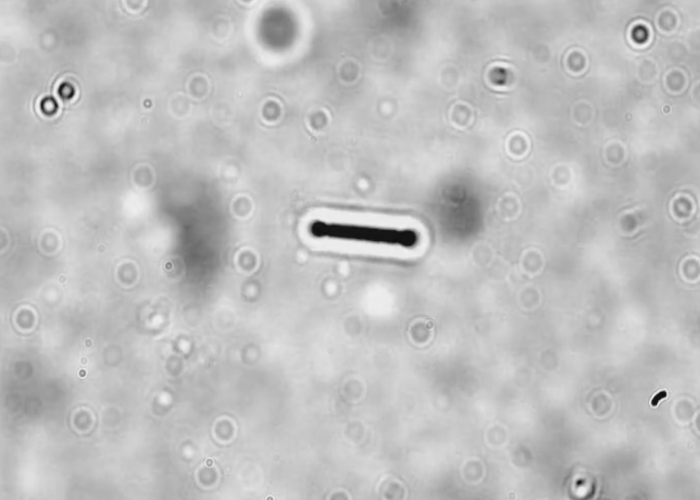
\includegraphics[width=\textwidth]{figures/method/static1.png}
\caption{A typical raw video frame.}\label{fig:origFrame}
\end{subfigure}\hspace{1em}%
\begin{subfigure}[3b]{0.40\textwidth}
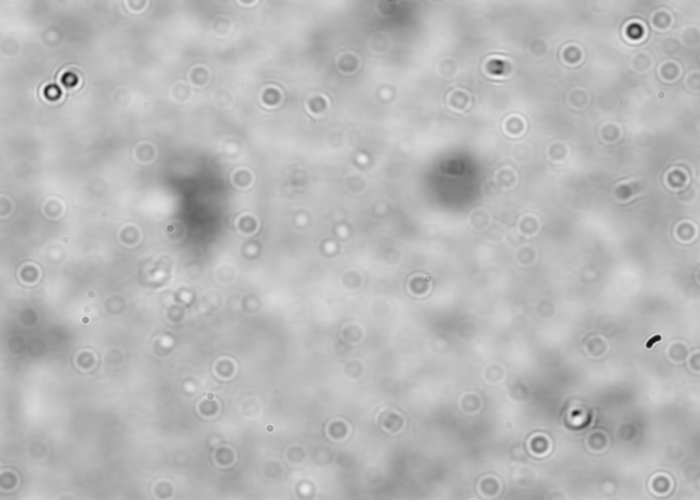
\includegraphics[width=\textwidth]{figures/method/static3.png}
\caption{The average frame $\bar{\mathbf{F}}$ from eq \ref{eq:averageFrame}.}\label{fig:averageFrame}
\end{subfigure} \\

\begin{subfigure}[3a]{0.4\textwidth}
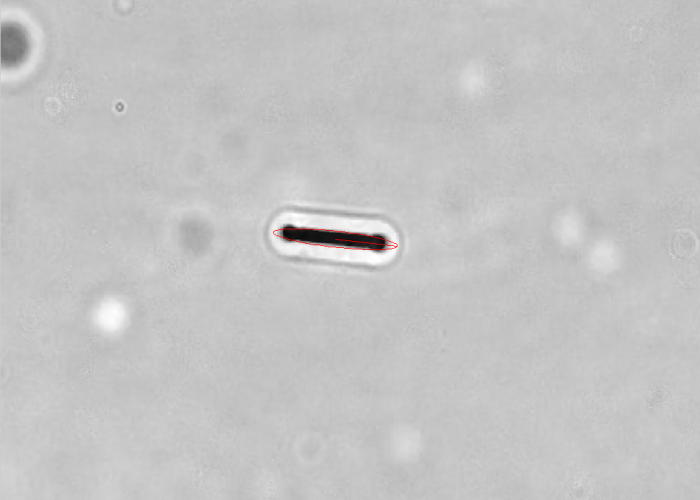
\includegraphics[width=\textwidth]{figures/method/static2.png}
\caption{The same frame after noise reduction}\label{fig:fixedFrame}
\end{subfigure}\hspace{1em}%
\begin{subfigure}[3a]{0.4\textwidth}
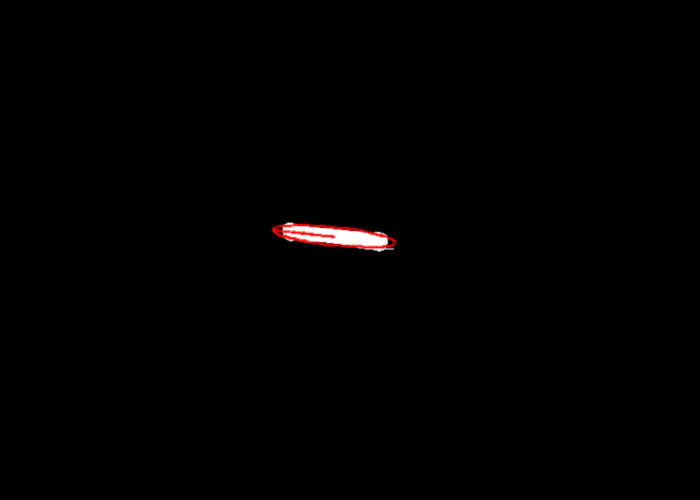
\includegraphics[width=\textwidth]{figures/method/edge.png}
\caption{After edge detection and ellipse fitting}\label{fig:edgeFrame}
\end{subfigure}

\caption{These pictures illustrate the most important step of the image analysis from raw image to estimated particle position. First the static noise from the average frame $\bar{\mathbf{F}}$}
\label{fig:detection}
\end{figure}

\section{Estimation of orientation}

The ellipsoid given by the fitting is then our best approximation of the projection in the $x$-$z$ plane. The projection of the particle along the $x$-axis and $z$-axis are found by
\begin{align} \label{eq:project}
p_x  &= l_e \sin(\phi_p) \\
p_z  &= l_e \cos(\phi_p) 
\end{align}

Here $p_x$ and $p_z$ are the $x$-axis and $z$-axis projection respectively.

To find the unit vector $\mathbf{n}$ we need to know the length of the particle. It was shown by Leal \cite{Leal} that the particle always spends a majority of its time aligned with the flow, ie aligned with the camera plane. This means that by finding the ellipse length $l_e$ every frame and finding the mode of the distribution we will find a good estimate of $L$. We find the orientation vector $\mathbf{n}$ from Section \ref{sec:jeffery} by normalizing the projections

\begin{subequations}\label{eq:normalize}
\begin{align}
n_x 	&= \frac{p_x}{L}, \\
n_z 	&= \frac{p_z}{L}, \\
n_y		&= \sqrt{1 - n_x^2 - n_z^2}.
\end{align}
\end{subequations}

This allows us to make comparisons between theory and measurement. Until this point the data analysis is the same as that in Johansson \cite{AntonThesis}.

\section{Width compensation}\label{sec:width_compensation}
We have assumed that the particle is a \emph{thin} rod so that the projection $\mathbf{p}$ onto the $x$ and $z$-axes give us an accurate estimate of $\mathbf{n}$. However, when we consider that our particle is 'thick' with length $l_e$ as well as width $w_e$ the actual unit vector we will be using in the above algorithms is $\mathbf{n}'$. The width of the particle will appear as an ellipse even when the particle is aligned completely with the $y$-axis. Looking at the points when $\phi = 0$, which are the points plotted on the surfaces of section and thus of the most 	interest, we find

\begin{equation}\label{eq:widthcomp}
\mathbf{n}' = \frac{p_z'}{L} = \frac{p_z\cos(\theta)  + D\sin(\theta)}{L} 
\end{equation}

which is illustrated in figure \ref{fig:lengtherror} for 4 different values of $\theta$. 

In order to compensate for the width of the particle we modify our projection equation \ref{eq:project} to

\begin{align}\label{eq:widthCompensation}
p_x  &= (l_e - w_e)\cdot \sin(\phi_p) \\
p_z  &= (l_e - w_e)\cdot \cos(\phi_p) 
\end{align}


This reduces the particles estimated length by $w_e$
\begin{figure}[H]
\centering
\includegraphics[width=0.6\textwidth]{figures/method/LengthError2.pdf}
\caption{Shows the incorrect projection vector $\mathbf{p}'$ we obtain from incorrectly assuming the particle is 'thin' in eq. \ref{eq:project}. The correct projection vector is highlighted in red. Shows four different $\theta$ angles at $\phi=0$.}\label{fig:lengtherror}
\end{figure} 



\section{Removing tracking errors}
\label{sec:brushing}
The tracking typically contains a few frames where the particle is not detected correctly due to being visually obstructed in some way. This causes to spikes in the data which complicates analysis. To make further theoretical analysis possible the data is corrected by removing such points manually. The basis for removal is a large discontinuity in the data, and many such points could be eliminated with algorithmic means. However in particular for $n_z$ it is very difficult to write an algorithm that catches all possible edge cases without having false positives. For example $n_z$ have peaks that make its derivative non continuous which means that a continuous derivative cannot be to exclude points. It's was found to be simpler to look at the analysis program and remove the points where the particle cannot be traced accurately due to noise. 

An example of data before and after correction can be seen in Figure \ref{fig:brushed} and all uncorrected data files of measurements used in this thesis are available at \url{http://goo.gl/jgzSXe}.

\begin{figure}[H]
\centering
\begin{subfigure}[3a]{0.40\textwidth}
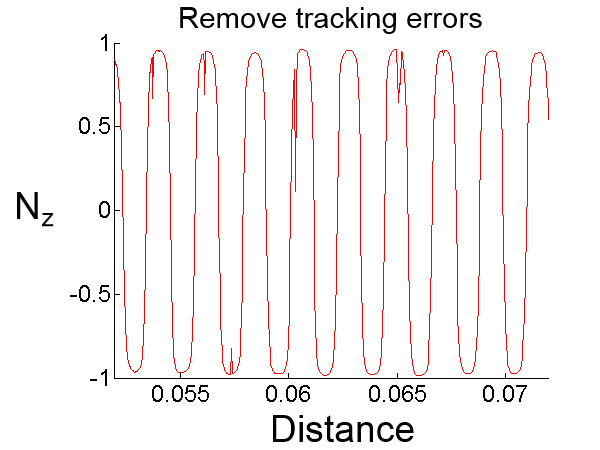
\includegraphics[width=\textwidth]{figures/method/Brushing1.png}
\caption{$n_x$ time series before correction.}\label{fig:prebrush}
\end{subfigure}\hspace{1em}%
\begin{subfigure}[3b]{0.40\textwidth}
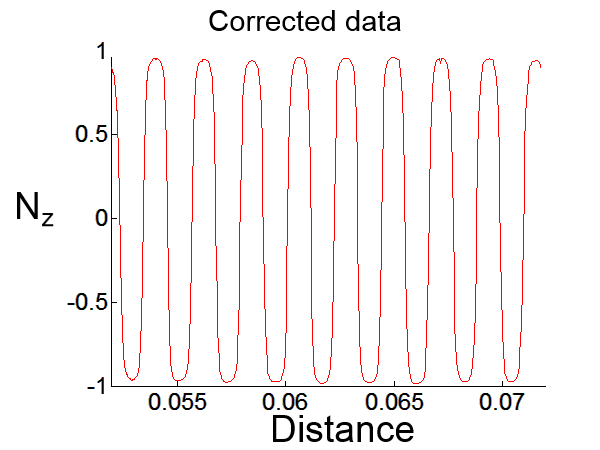
\includegraphics[width=\textwidth]{figures/method/Brushing2.png}
\caption{$n_x$ time series after correction.}\label{fig:postbrush}
\end{subfigure} \\
\caption{Shows screenshots from the software used to remove tracking errors for a time series of $n_z$ before and after removing points where a significant amount of noise disturbed the tracking.} \label{fig:brushed}
\end{figure}


\section{Estimating the winding numbers}
	\label{sec:windingEstimation}
As discussed in section \ref{sec:winding}, estimating the winding number for different types of orientational orbit for one particle allows for an estimation of $\epsilon$. In order estimate the winding number for a measured 
particle we must identify the two periods $\theta_1$ and $\theta_2$ from figure \ref{fig:windingDef}. 


\begin{figure}
\centering
\includegraphics[width=0.7\textwidth]{figures/method/nzNx0.pdf}
\caption{The stars are plotted at the same distances in the $n_x$ and $n_z$ plots. We see that zeros of $n_x$ and maxima of $n_z$ occur almost exactly at the same points.}
\label{fig:nzNx0}
\end{figure}

The maxima with the shorter period $\theta_2$ are located where $n_x = 0$ as is seen in figure \ref{fig:nzNx0}. We denote the set of these points $P_z$. The longer period $\theta_1$ is the periodicity of $P_z$, marked as red points in Figure\ref{fig:nzNx0}. To estimate the winding number we want to locate the maxima $M$ and minima $m$ in $P_z$ that occur with period $\theta_1$ in the same way we do to find $\theta_2$ in $n_z$. Unfortunately the height of peaks is noisy and there are few data points for each measurement as the channel is of finite length only allowing a few dozen flips. This means averaging cannot be used to reduce the noise.This means we have no algorithmic means to find $\theta_1$. 

Instead we select from $P_z$ a number of maxima $M_1, M_2 ... M_p$ and minima $m_1, m_2, ..., m_q$. We denote their index in $n_z$ as $I^M_1, I^M_2, 
..., I^M_p$ for the maxima and $I^m_1, I^m_2, ..., I^m_q$ for the minima. We can then find $\theta_1$ as the mean distance between successive maxima $\overline{d_M}$ and successive minima $\overline{d_m}$, 

\begin{align}
\overline{d_M} &= \frac{1}{p-1} \sum\limits_{j=1}^{p} I^M_{j+1} - I^M_{j} \\
\overline{d_m} &= \frac{1}{q-1} \sum\limits_{j=1}^{q} I^m_{j+1}- I^m_{j}\\
\hat{\theta_1}   &= \frac{\overline{d_M} + \overline{d_m}}{2}.
\label{eq:winding2}
\end{align}

In the case that we only have 1 maxima and minima eq. \ref{eq:winding2} can't be calculated so we assume that the distance between a maxima and minima is half a period, i.e.

\begin{equation}
\hat{\theta_1} = 2\left| I^M_1 - I^m_1 \right|
\end{equation}

\section{Matching data to theoretical orbits}
\label{sec:matchorbit}
To verify that the theoretical orbits from Section \ref{sec:jeffery} have been measured we want to match the measurements to theoretical orbits.

To find the best matching orbit from a Poincaré map for a measurement we again utilize $\mathbf{P}_z$, the points where $n_z$ peaks and $n_x=0$. We denote the length of $\mathbf{P}_z$ as $N$. We are concerned with matching them with the peaks from theoretical orbits.

%To find the best matching theoretical orbit we calculate the least square distance of $\mathbf{P_z}$ against the theoretical peaks for $\epsilon \in [0.01, 0.02, ..., 0.1]$ and for $\cos(\theta) \in [-1,1]$ 
%and for $\psi \in [-\frac{pi}{2},\frac{pi}{2}]$. 

To find the best matching theoretical orbit for a measurement we compute the least square distance between $\mathbf{P}_z$ and all orbits on all phase maps 
with $\epsilon$ in the range $\left[0.01, 0.02, ..., 0.1\right]$ for 200 consecutive initial $\psi$ (the $x$-axis on the Poincaré map). If we for each orbit denote 
the theoretical series of $n_z$ peaks as $\mathbf{Q}_z(\theta, \epsilon)$. We make sure that the length of $\mathbf{Q}_z(\theta, \epsilon)$ be twice that 
of $\mathbf{P}_z$ which guarantees that we always find the correct phase. We define $\mathbf{Q}_z(\theta, \epsilon, i)$ to be the $n_z$ series 
$\mathbf{Q}_z(\theta, \epsilon)$ starting at index $i$. We assign a score function $S(\theta, \epsilon, i)$ as

\begin{equation}
S(\mathbf{P}_z, \theta, \epsilon, i) = \frac{1}{N}\left| \mathbf{P}_z - \mathbf{Q}_z^{(i)}(\theta, \epsilon) \right|^2.
\end{equation}

\noindent An example experimental $P_z$ series matched to theoretical data is seen in Figure \ref{fig:particleB2match}.

\begin{figure}[H]
\centering
\includegraphics[width=0.7\textwidth]{figures/results/particleB/October_1_Particle_4_run_4match.pdf}
\caption{The upper figure shows the experimental $n_z$ peaks $\mathbf{P}_z$ and the theoretical peaks $\mathbf{Q}_z$ for the best matching orbit. The lower plot shows where what section of the theoretical time series was used for matching, ie what $i$ from section \ref{sec:matchorbit} was chosen.}
\label{fig:particleB2match}
\end{figure}



\noindent $\epsilon$ does not change for a particle over $r$ different measurements $\mathbf{P}_z^{(1)}, \mathbf{P}_z^{(2)}, ..., \mathbf{P}_z^{(r)}$, however the initial conditions $\theta$ and $i$ (the phase) do. So for each $\epsilon$ we find the best $\theta$ and $i$ using $\hat{S}(\mathbf{P}^{(j)}_z, \epsilon)$ 
\begin{equation}
\hat{S}(\mathbf{P}^{(j)}_z, \epsilon) =  \min(S(\mathbf{P}^{(j)}_z, \theta, \epsilon, i)) 
\end{equation}

\noindent and  then find the best $\epsilon$ using

\begin{eqnarray}
\epsilon_{best} = \min(\sum\limits_{j=1}^{r} \frac{\hat{S}(\mathbf{P}^{(j)}_z, \epsilon)^2).}{N^{(j)}}
\end{eqnarray}


It is important to note that this matching has a theoretical limitation. The asymmetry of our cylindrical particles is different from the asymmetry in the triaxial particles used in the theoretical models. The triaxial particles still have a rotational symetry for rotations of $\pi$ around any of the major/minor axes. This is not the case with the asymmetric cylindrical particles, which have no rotational symmetry. We therefore have to make the assumption that the difference between these two types of asymmetry is not significant and further theoretical work might reject this assumption.

% Refer to some matched plots once I have added those. I THINK basically everythig should already be in the saved plots and data folder. 


\chapter{Results}
The aim of these measurements is to show that the particles follow the Jeffery orbits and to show that they exhibit quasi-periodic or periodic motion for different initial conditions. In order to show that there are no significant disturbance we examine the reversal. If it reverts perfectly there has been no noise or inertial effects.

During the work of this thesis a large number of movies of particles have been recorded with gradual improvements to the setup primarily in terms of density matching, particle density (the number of particles per liquid volume)and  bubble elimination. In this section we present the data from two different particles. These were the only particles where there were good reversals for several stretches for both quasi periodic and periodic orbits. One referred to as particle A, the other as particle B. Particle A is approximately \unit[24]{$\mu m$} long so it has an aspection ratio $\lambda \approx 8$, particle B is approximately \unit[20.5]{$\mu m$} long so it has an aspection ratio $\lambda \approx 7$. The measurements in this section were done together with Alexander Laas.

We started each measurement at an approximate depth $D$ and at position $p_0 = (x_0, z_0)$ in the channel relative to the inlet on the right, closer to the pump. We have assumed that the shear is entirely in the $y$ direction when doing 	our theoretical analysis. This means the flow profile has to be almost entirely flat in the $z$-direction which it only is if the particle is close to the centre. Variations do occur but when are less than \unit[10]{$\mu$m} as is seen in figure \ref{fig:particleAsink}.

\newpage
\section{Measurements}
\subsection{Measurements of particle A}
Particle A was measured on October 11 in 2013. Two of the measurements retraced their orbits very well: measurement 1 and measurement 2 which can be seen in Figure \ref{fig:particleA1} and Figure \ref{fig:particleA2} respectively. Measurement 1 was started with initial condition $n_z \approx 0$ and showed quasi periodic behaviour with a periodic change in amplitude for $n_z$ peaks. Measurement 2 was started with initial condition $n_z \approx 1$ and showed periodic behaviour with very constant $n_z$ peaks. 

Other measurement had reversals where the orbit changed considerably, two examples are seen in Figure \ref{fig:particleA3} and \ref{fig:particleA4}. All measurement data for particle A can be found at \url{goo.gl/jgzSXe} where particle A is referred to as particle 2 from October 11. 


\subsubsection{Measurement 1}
\begin{figure}[H]
\begin{center}
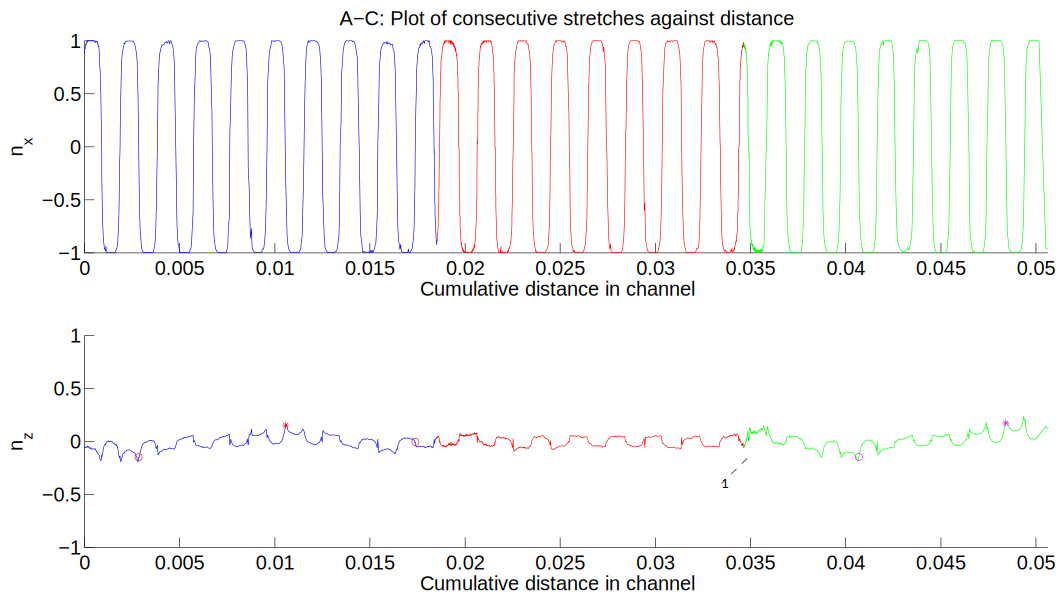
\includegraphics[width=0.7\textwidth]{figures/results/particleA/October_11_Particle_2_run_2_winding.pdf}
\end{center}
\caption{The $n_x$ and $n_z$ components of the particle for measurement 1 against cumulative distance in channel. Despite being very close to a centre orbit there is limited quasi-periodic behaviour as the peaks stay close to 0. The very flattened peaks compared to a low $n_z$ orbit in \ref{fig:orbitparams} are a result of the width compensation discussed in section \ref{sec:width_compensation}. This particle started $x_0 = 9.8 mm, z_0 = 8.9924 \mu m$ and $D \approx 90\mu$m. This is the same measurement as is used in Figure 6.20 in Laas thesis~\cite{alexanderThesis}}
\label{fig:particleA1}
\end{figure}


\subsubsection{Measurement 2}
\begin{figure}[H]
\begin{center}
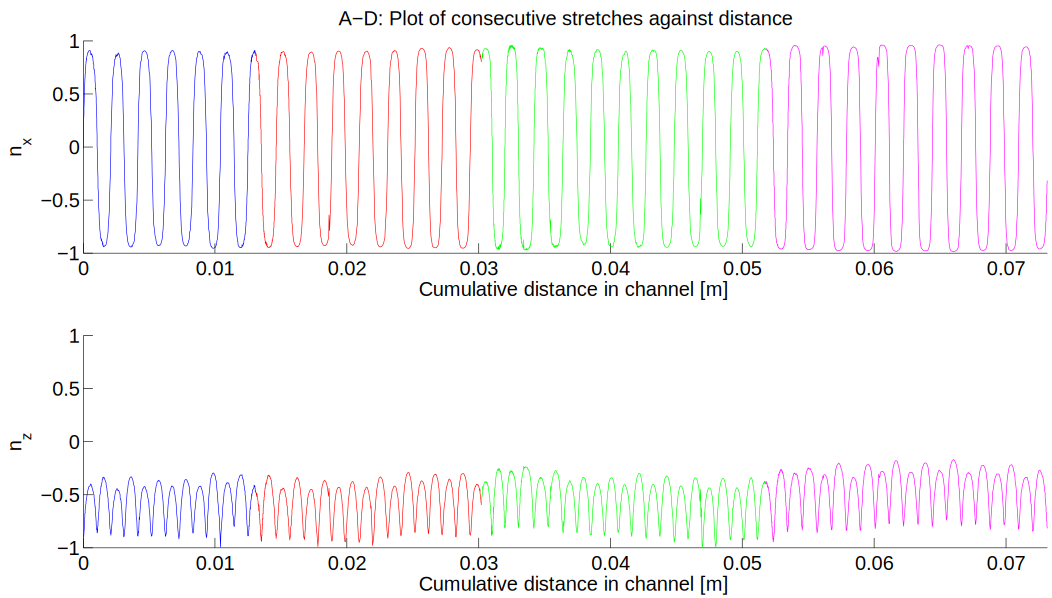
\includegraphics[width=0.7\textwidth]{figures/results/particleA/October_11_Particle_2_run_3_A.pdf}
\end{center}
\caption{The $n_z$ and $n_x$ components for measurement 2 against cumulative distance. The $n_z$ component is consistently close to 1 at the peaks. 
The particle started at $ x_0 = 26.0 \text{mm}, z_0 = 275\mu\text{m}, D\approx 105\mu$m. This figure is the same as Laas~\cite{alexanderThesis} Figure 6.21}
\label{fig:particleA2}
\end{figure}

\subsubsection{Measurement 3}
\begin{figure}[H]
\begin{center}
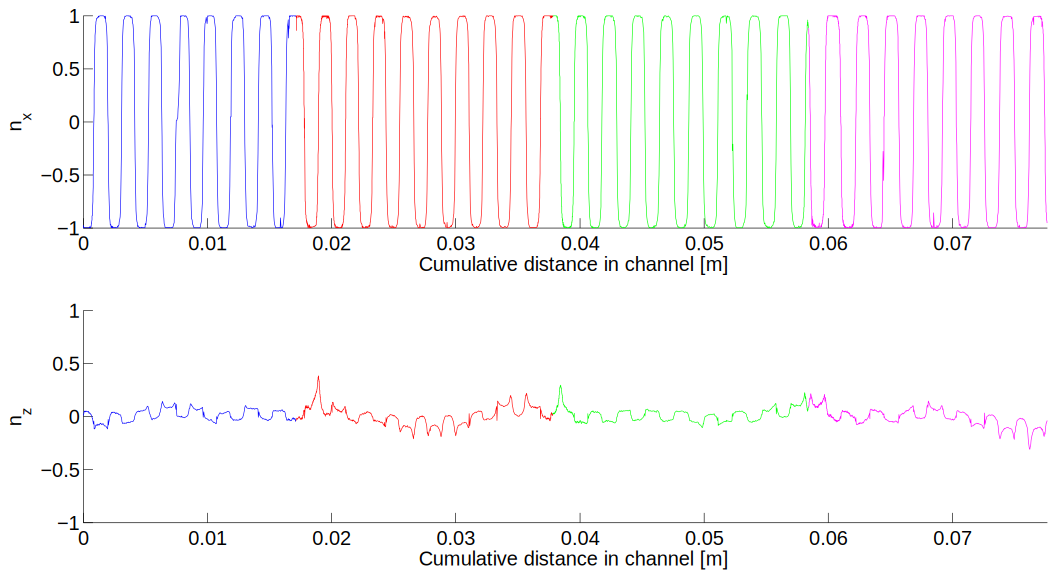
\includegraphics[width=0.7\textwidth]{figures/results/particleA/October_11_Particle_2_run_6_A.pdf}
\end{center}
\caption{The $n_z$ and $n_x$ components for measurement 3 against cumulative distance. The larger peaks that occur after the reversals are not the cause of a tracking error but can be seen clearly in the films. The reversal of the flow is started when the particle is next to the point marked (3) which is also where there is a change in $n_z$ component. The particle started at $ x_0 = 12.3 \text{mm}, z_0 = 160 \mu\text{m}, D \approx 100\mu$m.}
\label{fig:particleA3}
\end{figure}



\subsubsection{Measurement 4}
\begin{figure}[H]
\begin{center}
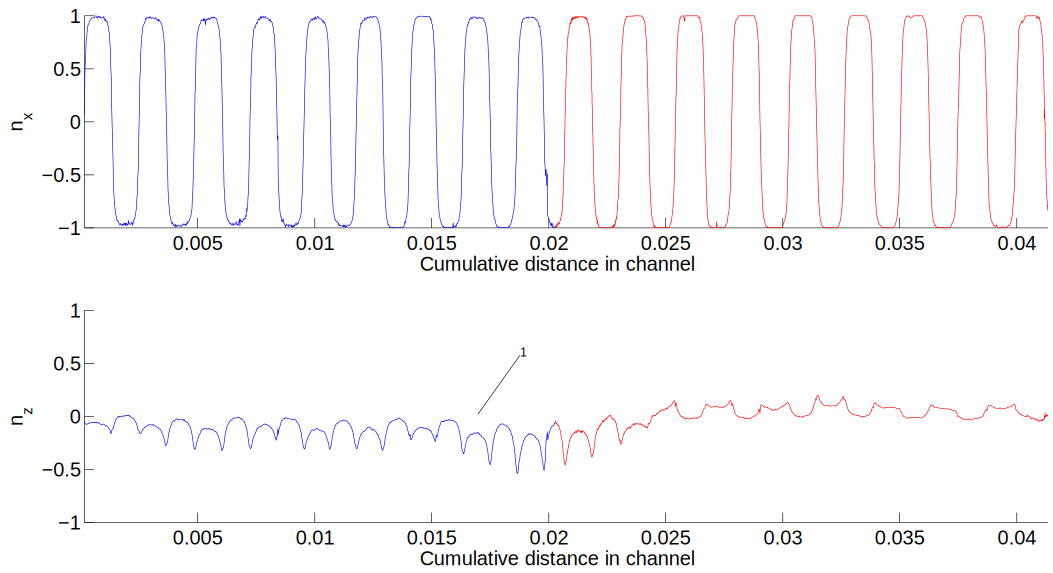
\includegraphics[width=0.8\textwidth]{figures/results/particleA/October_11_Particle_2_run_1_A.pdf}
\end{center}
\caption{The $n_z$ and $n_x$ components for measurement 4 against cumulative distance. The flow is reversed when the particle is at the point marked by (1) and we can see that the peaks around the reversal are larger than for the rest of the measurement. Started at $x_0 = 8.7 mm, z_0 = 16\mu m, D \approx 95\mu$m.}
\label{fig:particleA4}
\end{figure}

\subsubsection{Measurement 5}
\begin{figure}[H]
\centering
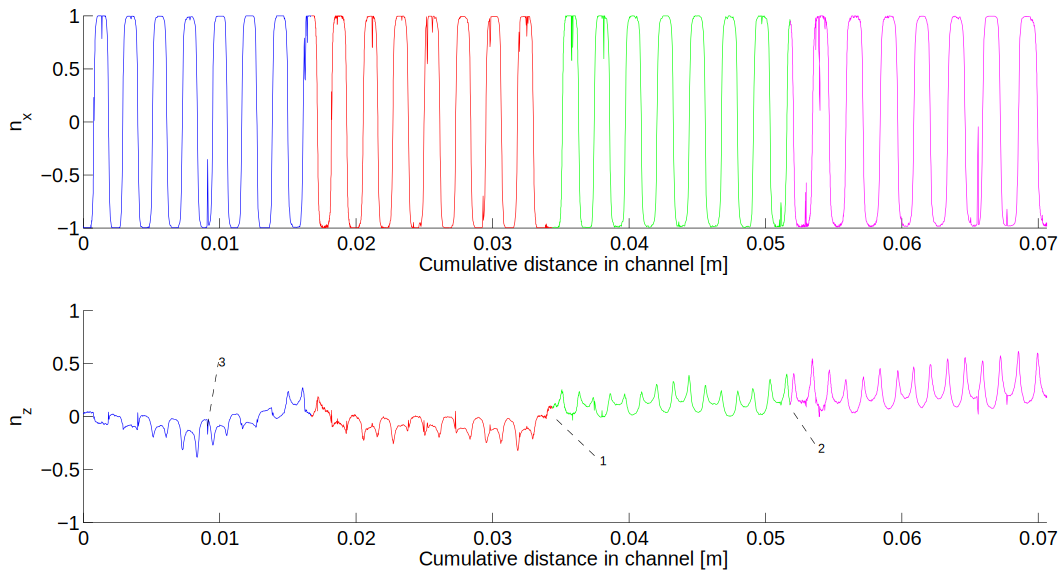
\includegraphics[width=0.8\textwidth]{figures/results/particleA/October_11_Particle_2_run_4_A.pdf}
\caption{The $n_z$ and $n_x$ components for measurement 5 against cumulative distance. At the point marked by (1) $n_z$ changes drastically at the reversal which occurs at the side of the channel closer to the pump. Although there is also some change in the orbit at the reversal marked by (2) it does not move comparably far on the S.O.S. There are a number of small peaks in the data such as the one indicated by (3) which is a consequence of insufficient removal of tracking errors, see Section \ref{sec:brushing}. The particle started at $x_0 = 10.7 mm, z_0 = 240 \mu m, D \approx 60\mu m$.}
\label{fig:particleA5}
\end{figure}

\subsection{Measurements of particle B}
Particle B was measured on October 1 2013. Particle B has four measurements for which most reversals showed little change in orbit. These are shown below in Figures \ref{fig:particleB1}, \ref{fig:particleB2}, \ref{fig:particleB3} and \ref{fig:particleB4}. There were also problematic measurements of particle B analogous to those for particle A, but they have not been included in this section for brevity. All measurement data for particle B can be found at \url{goo.gl/jgzSXe} where particle B is referred to as particle 4 from October 1. 

\subsubsection{Measurement 1}
\begin{figure}[H]
\begin{center}
\includegraphics[width=0.7\textwidth]{figures/results/particleB/October_1_Particle_4_run_2_winding.pdf}
\end{center}
\caption{The $n_z$ and $n_x$ components for measurement 1 against cumulative distance. The first two and the last two stretches the particle retraces its motion very closely during the reversals. In the reversal between these two reversals there is a large change in orbit which begins at (1) where the flow is starting to revert. This reversal occurs at the end of the channel closer to the pump. Starts at $ x_0 = 9.3$mm $,z_0 = 35\mu m, D \approx 100\mu m$. This is the same measurement as is used in Figures 6.2 and 6.4 in Laas thesis~\cite{alexanderThesis}}
\label{fig:particleB1}
\end{figure}
	


\subsubsection{Measurement 2}

\begin{figure}[H]
\begin{center}
\includegraphics[width=0.7\textwidth]{figures/results/particleB/October_1_Particle_4_run_4_A.pdf}
\end{center}
\caption{The $n_z$ and $n_x$ components for measurement 2 against cumulative distance. The orbit is mostly constant orbit with $n_z \approx 1$ at the peaks. The reversals at (1) and (3) both change the orbit slightly however the difference between the peaks is small and the best matched theoretical orbits in Figure\ref{fig:October1Particle4runs2and2Orbits} are similar before and after reversals. There is missing data at (2) and (4) where the particle was no able to be tracked. The particle started at $x_0 = 28.6$mm, $z_0 = 72\mu$m, $D = \approx 85\mu$m. This is the same measurement as is used in Figure 6.8 in Laas thesis~\cite{alexanderThesis}}
\label{fig:particleB2}
\end{figure}

\subsubsection{Measurement 3}
\begin{figure}[H]
\begin{center}
\includegraphics[width=0.7\textwidth]{figures/results/particleB/October_1_Particle_4_run_5_winding.pdf}
\end{center}
\caption{The $n_z$ and $n_x$ components for measurement 3 against cumulative distance. The initial condition is $n_z \approx 0$ and the sign changes periodically. Started at $x_0 = 2.7 mm, z_0 = 76\mu m, D \approx 90\mu$m. This is the same measurement as is used in Figures 6.10 and 6.12 in Laas thesis~\cite{alexanderThesis}}
\label{fig:particleB3}
\end{figure}


\subsubsection{Measurement 4}
\begin{figure}[H]
\begin{center}
\includegraphics[width=0.7\textwidth]{figures/results/particleB/October_1_Particle_4_run_3_winding.pdf}
\end{center}
\caption{The $n_z$ and $n_x$ components for measurement 4 against cumulative distance. While the changes are not large change in $n_z$ there is a periodic variations that could correspond to a sign preserving quasi-periodic orbit. Started at $x_0 = 12.9 mm, z_0 = 21\mu m, D \approx 85\mu$ m}
\label{fig:particleB4}
\end{figure}
\section{Diagnostic plots}

A number of diagnostic measurements were made for each particle to find possible problems with the setup. In this section we only show the diagnostic measurements from measurement 1 for particle A, and from measurement 2 for particle B but all diagnostic plots can be found at \url{http://goo.gl/jgzSXe}.


\begin{figure}[H]
\begin{center}
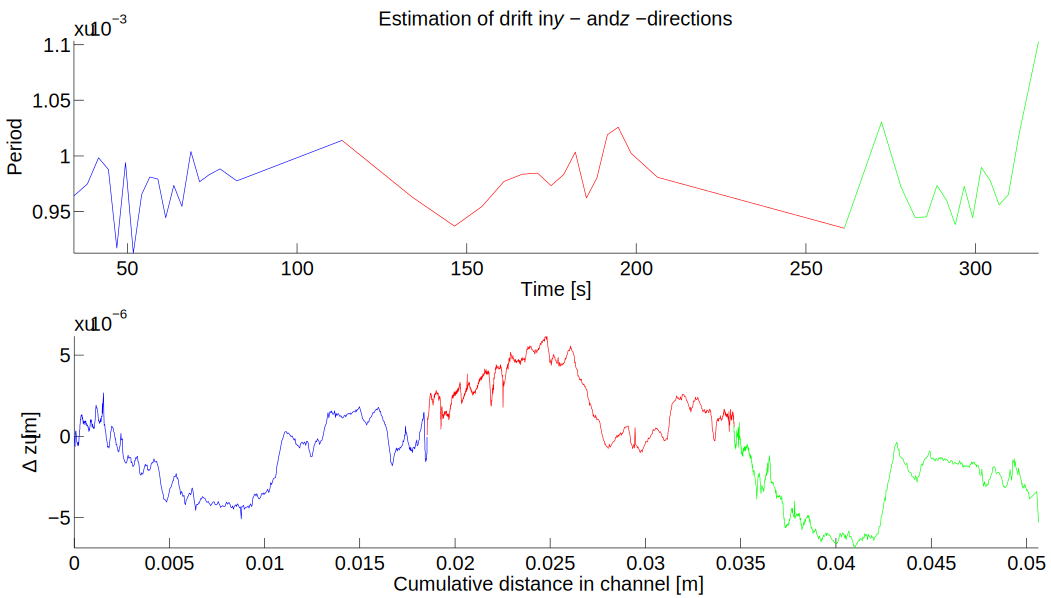
\includegraphics[width=0.7\textwidth]{figures/results/particleA/October_11_Particle_2_run_2_B.pdf}
\end{center}
\caption{The estimation of drift in $y$ and $z$ direction for Particle from measurement 1. Upper figure is the estimation of the sinking of the particle, the lower figure is the measured z position in the channel against cumulative distance. }
\label{fig:particleAsink}
\end{figure}

\begin{figure}[H]
\centering
\includegraphics[width=0.7\textwidth]{figures/results/particleB/October_1_Particle_4_run_4_B.pdf}	
\caption{The estimation of drift in $y$ and $z$ direction for Particle from measurement 1. Upper figure is the estimation of the sinking of the particle, the lower figure is the measured z position in the channel against cumulative distance.}
\label{fig:particleB2sinking}
\end{figure}



The center of mass movement in the direction perpendicular to the flow direction $x$ is seen in Figures \ref{fig:particleAsink} and \ref{fig:particleB2sinking}. Movement in the $y$ direction, i.e. sinking or floating, was measured by plotting the period of each flip against time as in the upper figure. The period here refers to the distance $\Delta_i$ between two successive zeros for $n_x$ relative to the first such distance $\Delta_0$. If there is no clear trend to higher or lower values it implies that there is little sinking or floating. 

The movement in the z coordinate is very small relative to the movements in the x direction. We can see that Z-direction movements along one stretch are on the order of $10\mu m$ compared to the x direction which is on the order of $2\cdot 10^4 \mu m$.The change in period was less than 20\% for all particles presented in this chapter.

The speed was plotted as a function of time to see how the flow reversed and if there were any problems with the pump. There is a noticeable difference between reversals that occur on the side of the channel and the side closer to the pump where on the reversal on the end of the channel further from the pump the speed drops to 0, increases for a short while and then goes back down to 0. This has been a consistent feature across all measurements.

\begin{figure}[H]
\begin{center}
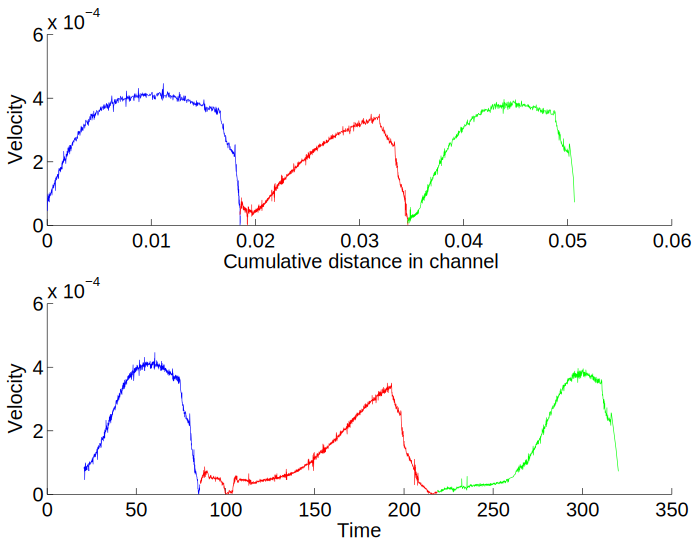
\includegraphics[width=0.7\textwidth]{figures/results/particleA/October_11_Particle_2_run_2_D.pdf}
\end{center}
\caption{The speed (note not the velocity) of the particle A from measurement 1 against cumulative distance in the upper figure and against time in the lower figure.}
\label{fig:particleAspeed}
\end{figure}


\begin{figure}[H]
\begin{center}
\includegraphics[width=0.7\textwidth]{figures/results/particleB/October_1_Particle_4_run_2_D.pdf}
\end{center}
\caption{The speed (note not the velocity) of particle B from measurement 2 against distance in the upper figure and against time in the lower figure. In the plot against time there is an extra dip to 0 at around $t=150$ and $t=400$. This occurs at the end of channel further away from the pump.}
\label{fig:particleB1speed}
\end{figure}


\subsection{Reversals}
In order to show that the dynamics of the particle revert when the flow is reversed we plot the components of $\mathbf{n}$ against distance in the channel. The first reversal from measurement 1 for particle A is seen in Figure \ref{fig:particleAreversegood}. There is very good agreement along the entire length of the channel only at the very end does is there a difference larger than the margin of error. The same plot is made from the second reversal from measurement 5 in Figure \ref{fig:particleABadReversal}. Here the particle changes orbit drastically at the reversal while being stable before and after. 

\begin{figure}[H]
\begin{center}
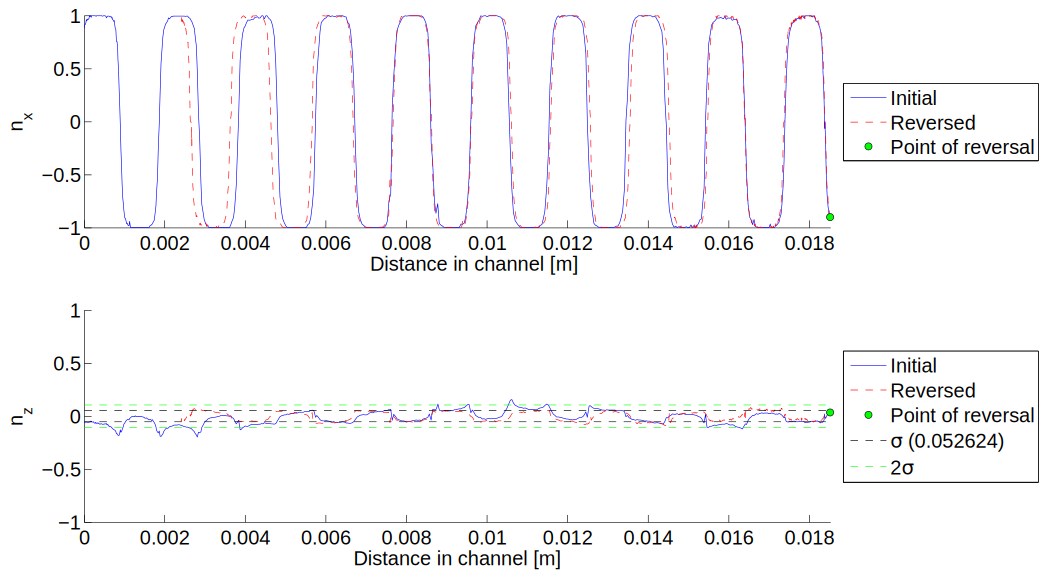
\includegraphics[width=0.7\textwidth]{figures/results/particleA/October_11_Particle_2_run_2_C01.pdf}
\end{center}
\caption{Shows $n_x$ and $n_x$ first and second stretches from Measurement 1, seen in Figure \ref{fig:particleA1} but against the actual position in the channel as opposed to cumulative distance. There is an almost perfect match along the entire channel for $n_x$ and only small disagreement for $n_z$. The dashed lines indicate the error margins for detecting $n_z=0$. This figure is the same as can been seen in Laas\cite{alexanderThesis} Figure 6.21}
\label{fig:particleAreversegood}
\end{figure}

 \begin{figure}[H]
 \centering
 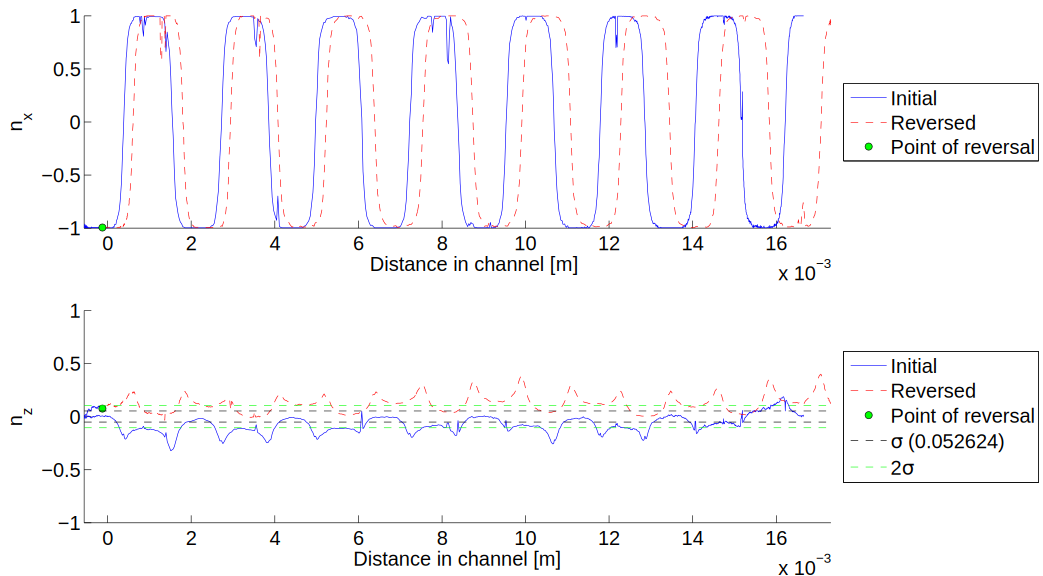
\includegraphics[width=0.8\textwidth]{figures/results/particleA/October_11_Particle_2_run_4_C02.pdf}
 \caption{$n_x$ and $n_z$ from Figure \ref{fig:particleA5} for the second and third stretch plotted against actual distance instead of commutative distance. The reversal occurs at the left and although there is some moderate agreement in $n_x$ the match in $n_z$ is non existant from the very start.}
 \label{fig:particleABadReversal}
 \end{figure}

\section{Match to theoretical orbits}
\subsection{Particle A}
Particle A is approximately \unit[24]{$\mu m$} long so it has a $\lambda$ close to 8 and the closest match for the asymetry is $\epsilon = 0.02$. \ref{fig:particleA1}


Using the algorithm described in section \ref{sec:matchorbit} we match the data from measurement 1 and 2 for particle A to find the closest matching $\epsilon$ and the best matching orbits. This is shown in Figure\ref{fig:particleAOrbitFit}. We can see that particle A is in a quasi-periodic circular orbit during measurement 1, it is matched to the lines indicating A B and C for the first, second and third stretches respectively.  After being shifted by the optical tweezers, particle A followed a periodic orbit during measurement 2. Measurement 2 is matched to the orbits D, E, F and G for the first, second, third and fourth stretches respectively. The stretches that do not have winding numbers listed in the figures had orbits that did not have enough variation in $n_z$ peaks to try to estimate a winding number. 

\begin{figure}[H]
\begin{center}
\includegraphics[width=\textwidth]{figures/results/orbitmatches/AmapAdded.pdf}
\end{center}
\caption{Black lines show the Poincaré map of the Jeffery's equations for $\lambda = 8$ and $\epsilon = 0.02$. The measured $\lambda$ was $8.2 \pm 0.1$. The orbits of the best fit theoretical fits to measurements are highlighted stretch by stretch. None of the orbits for this particle had any large variation despite being very close to $n_z=0$. The winding numbers are within 50\% of the estimates but both are too low, suggesting that the $\epsilon$ might be too low.}
\label{fig:particleAOrbitFit}
\end{figure}

\subsection{Particle B}

The same procedure is repeated for particle B using the data from measurement 1,2, 3 and 4. To make the graph less cluttered it is split into two figures, Figure \ref{fig:October1Particle4runs2and2Orbits} for measurement 1 and 2 and Figure \ref{fig:October1Particle4_runs3and5Orbits} for measurement 3 and 4. We can see that particle B is in a quasi-periodic circular orbit , it is matched to the lines indicating A B and C for the first, second and third stretches respectively.  After being shifted by  the optical tweezer particle A followed a periodic orbit during measurement 2. Measurement 2 is matched to the orbids D, E, F and G for the first, second, third and fourth stretches respectively. 

\begin{figure}[H]
\centering
\includegraphics[width=\textwidth]{figures/results/orbitmatches/Bmap1Added.pdf}
\caption{Black lines show the Poincaré map of the Jeffery's equations for $\lambda = 7$ and $\epsilon=0.04$, the estimate of $\lambda$ from measurement was $6.7 \pm 0.1$. The highlighted orbits are the best fits to the stretches from measurements 1 and 2, A-D from measurement 1 and E-I from measurement 2.}
\label{fig:October1Particle4runs2and2Orbits}
\end{figure}


\begin{figure}[H]
\centering
\includegraphics[width=\textwidth]{figures/results/orbitmatches/Bmap1Added.pdf}
\caption{Black lines show the Poincaré map of the Jeffery's equations for $\lambda = 7$ and $\epsilon = 0.04$. the estimate of $\lambda$ from measurement was $6.7 \pm 0.1$ . The highlighted orbits are the best fits to the stretches from measurements 3 and 4.}
\label{fig:October1Particle4_runs3and5Orbits}
\end{figure}





\chapter{Discussion}
Looking at figures \ref{fig:October1Particle4_runs3and5Orbits}, \ref{fig:October1Particle4runs2and2Orbits} and \ref{fig:particleAOrbitFit} we find all three types of orbits discussed in section \ref{sec:winding} and their winding numbers for the orbits where we can measure it also agree well with our theoretical predictions. This is however only for the stretches that do work well, and even in those measurements there are many reversals where there are large differences before and after such as in figure \ref{fig:particleABadReversal}. 

In general orbits with higher $n_z$ have very periodic orbits, whereas low $n_z$ do not. 

We see four major problems in the data 

\begin{enumerate}
\item Sinking
\item Bad reversals
\item Too few flips to clearly estimate winding number
\item Unexplained changes in orbit
\end{enumerate}

\section{Sinking}
One of the major problems with this setup compared to the previous setup is the density matching, given a density mismatch of $\unit[0.05]{g/ml}$ we find using \ref{eq:fallingSphere} a falling speed of $\frac{2}{9} \frac{0.05 \cdot 9.82 \cdot (10^{-5})^2}{2.4\cdot 10^-3} = \unit[4.9\cdot10^3 ]{\mu m/s}$. In earlier measurements the pump speed was $\unit[3]{\mu l/minute}$ and the particle were 60\% larger, which meant the sinking occurred more than twice as long and twice as fast which meant it was a larger problem. Even now though it can be noticeably as in longer measurements such as in figures \ref{fig:particleB2} and \ref{fig:particleB2sinking}.

\section{Reversals}
Almost every measurement with several stretches will have on reversal where the particle noticeably changes orbit. This can been seen figures \ref{fig:particleA5}, \ref{fig:particleA4} and \ref{fig:particleB1}. While there is a trend that bad reversals occur at he end further from the channel there are many exceptions to this. There are many cases where the orbit begins to change just as the flow is starting to reverse, such as in figure \ref{fig:particleA4} so a possible culprit would then be that reversals occur too rapidly.



\subsection{Velocity behaviour}
A possible cause of bad reversals are too rapid reversals and to prevent this the reversals are staggered. At the start of a reversal the infusion/withdrawal rate is reduced to 50\% for 10 seconds, then stopped completely for 10 seconds and reverted at 50\% for another 10 seconds before resuming at full speed.

Possibly increasing this staggering on the first part might make a difference, but if we look at the plot of the 
speed of the particle in figure \ref{fig:particleAspeed} and \ref{fig:particleB1speed} we see that after a rather 
sharp decline in speed the acceleration is very slow. Almost all of this acceleration occurs while the pump is 
infusing or withdrawing at a fixed rate. Now the liquid accelerating while the pump rate constant suggests that there 
is a noticeably expansion in the channel. To verify this we can look more closely at he speed graphs 
\ref{fig:particleAspeed} and \ref{fig:particleB1speed}.

If we have an expanded/contracted channel it should have different effects on different sides of the channel. We 
expect that on the side closer to the pump the expanding channel will simply absorb part of the fluid infused causing 
a slowed acceleration but it would start more or less right as the pump starts infusing/withdrawing. Meanwhile on the 
far end of the channel the 'extra' fluid in the channel could be withdrawn before any pressure is felt on the far 
side. This would cause a delay where there is no acceleration for some while after the pump started acceleration. 

This behaviour is exactly what we see in all speed plots like \ref{fig:particleAspeed} and \ref{fig:particleB1speed}, 
on reversals on the far end there is a second dip where the particle starts at $\left|v\right|=0$ for some extra 
seconds. On the end closer to the pump this never occurs. 

An earlier theory for the delay would be an offset in the pump, for example a distance between the syringe handle and the pump holder which would need to be traversed, but this would occur at both ends of the channel and would not explain the very long acceleration of the fluid. 

\section{Winding number matching}
While using the score function $\hat{S}$ to find the closest matching orbit is useful, it only gives the best fit and 
does not actually show that the orbit is close (just more close than the other ones). Instead the best tool for 
validating, or dismissing, a matched orbit and an estimated $\epsilon$ is the winding number for the orbits where 
this can be done. If we look at figure \ref{fig:windingdifferent} we see that the difference in winding number of the 
same $\theta$ is on the order of a factor 2 between $\epsilon = 0.01$ and $\epsilon = 0.05$ for circular orbits, and 
still quite noticeably different between $\epsilon = 0.05$ and $\epsilon = 0.10$, especially where the change from 
circular to bent orbit occurs. 

When we look instead at orbits for large $\left| n_z \right|$ like in figure 
\ref{fig:October1Particle4runs2and2Orbits} or for $n_z \approx \psi \approx 0$ like orbit B in figure 
\ref{fig:particleAOrbitFit} there is not much information to extract. The orbits for different $\epsilon, \lambda$ 
and $i$ all largely the same, the differences are too small for us to reliably detect. This creates a problem for 
detecting particles with very small $\epsilon$. For $n_z$ that are very small, we cannot distinguish the orbits for a 
small $\epsilon$ particle with higher $\psi$ orbit for a high $\epsilon$ particle with a low $\psi$ orbit. For higher 
$n_z$ we cannot distinguish straight lines from straight lines. And in the intermediary we are unable to detect a $w 
> 20$, at best finding a sloping $n_z$ which might just be undesired reversals. Particle A has several orbits that 
are matched in the intermediary circular $n_z$ region which we can distinguish from $\epsilon = 0$ but we can not 
estimate the winding number especially well as we barely have a half period. If we indeed had a circular orbit with 
$w = 19.5$ as predicted we need to use the end point 


\section{Unexplained behaviours}
In a number of measurements there are changes in orbit for which we have no good explanation. For example in figure \ref{fig:particleA5} the second reversal is cmpletely sharp, the orbit virtually instantly changes, completely 'forgetting' the previous orbit. Why does this occur with the same particle, the same setup, seemingly the same conditions that produce the excellent reversals in figure \ref{fig:particleA1}. The only difference is the z coordinate, yet figure \ref{fig:particleA3} was measured at a similar z and showed very few odd behaviours. This could be explained


\section{Goodness of fit}
 The method for matching the data to a theoretical orbit described in \ref{sec:matchorbit} finds the best fit but it is important to know how good of a fit. A flat fitness curve would mean a very small change in the data could lead to a very large change in our matched orbit. To determine the goodness of fit we vary the three parameters separately and find the best fit for the other two parameters. In Figure \ref{fig:asymVariation} we find the best matching orbits for Particle A for asymmetries ranging from 0 to 0.2. We see that there is a clear minima around $\epsilon = 0.02$ implying that it is a good fit.
 
 In Figure \ref{fig:orbitVariation} the match of stretch 1 from measurement 1 of particle A is matched. We use the best matching asymmetry, match for orbits from the center of the pointcare map to the top. For each orbit we find the best starting position (the initial $\psi$). The result is a steady slope down to the correct orbit suggesting that this variable also had a clear best value that was chosen. 
 
 The best In Figure \ref{fig:initVariation} we use the best matching 		asymmetry and orbit for stretch 1 from measurement 1 of particle A, and the starting position (initial $\psi$) is varied over 1 full period. The relatively flat slope suggests that this parameter while certainly improving the fit slightly is not as important as the other two parameters. 
 
 \begin{figure}[H]
 \begin{center}
 \includegraphics[width=0.7\textwidth]{figures/results/particleA/A_assymVariation.pdf}
 \end{center}
 \caption{We see how the difference between the theoretical $n_z$ and all the measured  $\widetilde{n_z}$ for all measurements of particle A for different asymmetries $\epsilon$. For each asymmetry we find the orbit and the initial $\psi$ with the smallest distance for each stretch. We see that there is a clear minima around $\epsilon = 0.02$}
 \label{fig:asymVariation}
 \end{figure}
 
 \begin{figure}[H]
 \begin{center}
 \includegraphics[width=0.7\textwidth]{figures/results/particleA/A_orbitVariation.pdf}
 \end{center}
 \caption{The difference between the theoretical $n_z$ and the measured $\widetilde{n_z}$ for the first stretch of the measurement 1 for particle A (seen in figure \ref{fig:particleA1})with the best asymmetry for different orbits. .}
 \label{fig:orbitVariation}
 \end{figure}
 
 
 \begin{figure}[H]
 \begin{center}
 \includegraphics[width=0.7\textwidth]{figures/results/particleA/A_posVariation.pdf}
 \end{center}
 \caption{The difference between the theoretical $n_z$ and the measured $\widetilde{n_z}$ for the first stretch of the first measurement for particle A. The best orbit and best asymmetry are chosen, but different initial conditions are tested. }
 \label{fig:initVariation}
 \end{figure}
 



\chapter{Conclusion}
The Jeffery orbits are frequently used across scientific fields but thus far there has been few experimental studies 
of the orientational dynamics. In particular the quasi-periodic and chaotic orbits have only been studied experimentally
by Einarsson \emph{et al.}~\cite{JonasExperiment} and Mishra \emph{et al.}~\cite{Mishra}.
The goal of the thesis was to verify the theoretical predictions of Yarin \emph{et al.}~\cite{Yarin} and Hinch,Leal~\cite{Leal} and to show that the same particle could exhibit quasi-periodic and periodic behaviour for different initial conditions.

% % Introduce the experiment

There are several measurements that agree well with theoretical models by comparing using both the phase map matching and the winding number estimation. Furthermore, for several particles we have found that different initial conditions exhibit different behaviour. 
From almost constant to being quasi-periodic with a large regular variation. We can therefore conclude that we have measured the
orbits predicted by Yarin \emph{et al.}~\cite{Yarin} and Hinch, Leal~\cite{Leal}.

The time reversibility of the system is unreliable, for some measurements the dynamics revert very well, and for others it does not. 
We have not understood fully what causes this type of unpredictability that can occur for the same particle only 
minutes apart. The primary focus of future efforts should be understanding and correcting whatever issues cause the 
reversals to be so unreliable. It is possible that the time reversal can be improved by attempting to somehow increase the viscosity of the liquid
without changing the optical index. Another or by slowing down reversals. Another possibility is limiting the 
significant expansion and contraction of the channel that seems to occur.

The automated tracking was useful, but with the increased flow speed during measurements, as well as the smaller particles, 
there a better predictive model is needed in order to not lose the particle during reversals. The tracking is also less necessary 
measurements take significantly less time., However if significantly slower reversals become the preferred way of improving 
time reversibility then the tracking may be more useful.


%\section{$\mathbf{\lambda}$ of about 6}
%These are the particles with a $\lambda = 6 \pm 0.5$
%\subsection{Particle 1}

\begin{figure}[H]
\centering
\includegraphics[width=0.8\textwidth]{Images/Particle 1/Particle1.pdf}
\caption{Particle 1: $ \lambda: 6.1591$Depth: 160 out of $200 \mu $ m}
\end{figure}

\begin{figure}[H]

\centering

\includegraphics[width=0.8\textwidth]{Images/Particle 1/Stretch1.pdf}

\end{figure}

\begin{figure}[H]

\centering

\includegraphics[width=0.8\textwidth]{Images/Particle 1/Stretch2.pdf}

\end{figure}

\subsection{Particle 4}

\begin{figure}[H]
\centering
\includegraphics[width=0.8\textwidth]{Images/Particle 4/Particle4.pdf}
\caption{Particle 4: At around 10 minutes, pretty big "jump" in channel flow. $ \lambda: 12.7745$Depth: 140 out of $200 \mu $ m}
\end{figure}

\begin{figure}[H]
\centering
\includegraphics[width=0.8\textwidth]{Images/Particle 4/Stretch1.pdf}
\end{figure}


\begin{figure}[H]
\centering
\includegraphics[width=0.8\textwidth]{Images/Particle 4/Stretch2.pdf}
\end{figure}


\subsection{Particle 11}

\begin{figure}[H]
\centering
\includegraphics[width=0.8\textwidth]{Images/Particle 11/Particle11.pdf}
\caption{Particle 11: At around 7:03, possible interaction with dirt in channel. $ \lambda: 5.9638$Depth: 180 out of $200 \mu $ m}
\end{figure}

\begin{figure}[H]
\centering
\includegraphics[width=0.8\textwidth]{Images/Particle 11/Stretch1.pdf}
\end{figure}

\begin{figure}[H]
\centering
\includegraphics[width=0.8\textwidth]{Images/Particle 11/Stretch2.pdf}
\end{figure}


\subsection{Particle 13}
\begin{figure}[H]
\centering
\includegraphics[width=0.8\textwidth]{Images/Particle 13/Particle13.pdf}
\caption{Particle 13: At around 4:15 there is a big jump in the flow at reversal. $ \lambda: 5.5457$Depth: 140 out of $200 \mu $ m}
\end{figure}

\begin{figure}[H]
\centering
\includegraphics[width=0.8\textwidth]{Images/Particle 13/Stretch1.pdf}
\end{figure}


\subsection{Particle 16}
\begin{figure}[H]
\centering
\includegraphics[width=0.8\textwidth]{Images/Particle 16/Particle16.pdf}
\caption{Particle 16: $ \lambda: 6.2917$Depth: 120 out of $200 \mu $ m}
\end{figure}

\begin{figure}[H]

\centering

\includegraphics[width=0.8\textwidth]{Images/Particle 16/Stretch1.pdf}

\end{figure}

\begin{figure}[H]

\centering

\includegraphics[width=0.8\textwidth]{Images/Particle 16/Stretch2.pdf}

\end{figure}



\subsection{Particle 22}

\begin{figure}[H]


\centering
\includegraphics[width=0.8\textwidth]{Images/Particle 22/Particle22.pdf}
\caption{Particle 22: $ \lambda: 11.6767$Depth: 160 out of $200 \mu $ m}

\end{figure}

\begin{figure}[H]

\centering

\includegraphics[width=0.8\textwidth]{Images/Particle 22/Stretch1.pdf}

\end{figure}

\begin{figure}[H]

\centering

\includegraphics[width=0.8\textwidth]{Images/Particle 22/Stretch2.pdf}

\end{figure}

\subsection{Particle 23}

\begin{figure}[H]
\centering
\includegraphics[width=0.8\textwidth]{Images/Particle 23/Particle23.pdf}
\caption{Particle 23: $ \lambda: 5.6106$Depth: 80 out of $200 \mu $ m}
\end{figure}

\begin{figure}[H]
\centering
\includegraphics[width=0.8\textwidth]{Images/Particle 23/Stretch1.pdf}
\end{figure}




%
%\section{$\mathbf{\lambda}$ of about 6}
%These are the particles with a $\lambda = 7 \pm 0.5$
%\subsection{Particle 2}

\begin{figure}[ H]

\caption{Particle 2: $ \lambda: 13.9227$Depth: 30 out of $200 \mu $ m}

\centering

\includegraphics[width=0.8\textwidth]{Images/Particle 2/Particle2.pdf}

\end{figure}

\begin{figure}[ H]

\centering

\includegraphics[width=0.8\textwidth]{Images/Particle 2/Stretch1.pdf}

\end{figure}

\begin{figure}[ H]

\centering

\includegraphics[width=0.8\textwidth]{Images/Particle 2/Stretch2.pdf}

\end{figure}

\begin{figure}[ H]

\centering

\includegraphics[width=0.8\textwidth]{Images/Particle 2/Stretch3.pdf}

\end{figure}

\begin{figure}[ H]

\centering

\includegraphics[width=0.8\textwidth]{Images/Particle 2/Stretch4.pdf}

\end{figure}

\begin{figure}[ H]

\centering

\includegraphics[width=0.8\textwidth]{Images/Particle 2/Stretch5.pdf}

\end{figure}

\begin{figure}[ H]

\centering

\includegraphics[width=0.8\textwidth]{Images/Particle 2/Stretch6.pdf}

\end{figure}


\subsection{Particle 7}

\begin{figure}[ H]

\caption{Particle 7: $ \lambda: 27.4694$Depth: 20 out of $200 \mu $ m}

\centering

\includegraphics[width=0.8\textwidth]{Images/Particle 7/Particle7.pdf}

\end{figure}


\subsection{Particle 18}

\begin{figure}[ H]

\caption{Particle 18: Unclear. There are several possible interactions around 6 minutes but neither is all too clear. Also the second turn is overall quite jumpy$ \lambda: 14.3568$Depth: 20 out of $200 \mu $ m}

\centering

\includegraphics[width=0.8\textwidth]{Images/Particle 18/Particle18.pdf}

\end{figure}

\begin{figure}[ H]

\centering

\includegraphics[width=0.8\textwidth]{Images/Particle 18/Stretch1.pdf}

\end{figure}

\begin{figure}[ H]

\centering

\includegraphics[width=0.8\textwidth]{Images/Particle 18/Stretch2.pdf}

\end{figure}


\subsection{Particle 19}

\begin{figure}[ H]

\caption{Particle 19: At around 0:50 there is an uneven vertical flow "surging" the particle down. $ \lambda: 13.795$Depth: 120 out of $200 \mu $ m}

\centering

\includegraphics[width=0.8\textwidth]{Images/Particle 19/Particle19.pdf}

\end{figure}

\begin{figure}[ H]

\centering

\includegraphics[width=0.8\textwidth]{Images/Particle 19/Stretch1.pdf}

\end{figure}

\begin{figure}[ H]

\centering

\includegraphics[width=0.8\textwidth]{Images/Particle 19/Stretch2.pdf}

\end{figure}



 


\subsection{Particle 20}

\begin{figure}[ H]

\caption{Particle 20: At 5:22 collides with large "debris" on channel floor. $ \lambda: 13.5864$Depth: 150 out of $200 \mu $ m}

\centering

\includegraphics[width=0.8\textwidth]{Images/Particle 20/Particle20.pdf}

\end{figure}

\begin{figure}[ H]

\centering

\includegraphics[width=0.8\textwidth]{Images/Particle 20/Stretch1.pdf}

\end{figure}



\subsection{Particle 24}

\begin{figure}[ H]

\caption{Particle 24: $ \lambda: 14.3715$Depth: 60 out of $200 \mu $ m}

\centering

\includegraphics[width=0.8\textwidth]{Images/Particle 24/Particle24.pdf}

\end{figure}

\begin{figure}[ H]

\centering

\includegraphics[width=0.8\textwidth]{Images/Particle 24/Stretch1.pdf}

\end{figure}

\begin{figure}[ H]

\centering

\includegraphics[width=0.8\textwidth]{Images/Particle 24/Stretch2.pdf}

\end{figure}

%
%\section{Other particles}
%\subsection{Particle 3}

\begin{figure}[H]

\includegraphics[width=0.8\textwidth]{Images/Particle 3/Particle3.pdf}

\caption{Particle 3:  $ \lambda: 19.5489$ Depth: 140 out of $200 \mu $ m}

\centering

\end{figure}

\begin{figure}[H]

\centering

\includegraphics[width=0.8\textwidth]{Images/Particle 3/Stretch1.pdf}

\end{figure}


\subsection{Particle 5}

\begin{figure}[H]

\includegraphics[width=0.8\textwidth]{Images/Particle 5/Particle5.pdf}

\caption{Particle 5:  $ \lambda: 15.2445$ Depth: 160 out of $200 \mu $ m}

\centering

\end{figure}

\begin{figure}[H]

\centering

\includegraphics[width=0.8\textwidth]{Images/Particle 5/Stretch1.pdf}

\end{figure}

\begin{figure}[H]

\centering

\includegraphics[width=0.8\textwidth]{Images/Particle 5/Stretch2.pdf}

\end{figure}


\subsection{Particle 6}

\begin{figure}[H]
\includegraphics[width=0.8\textwidth]{Images/Particle 6/Particle6.pdf}
\caption{Particle 6:  $ \lambda: 17.3351$ Depth: 150 out of $200 \mu $ m}
\centering

\end{figure}

\begin{figure}[H]

\centering

\includegraphics[width=0.8\textwidth]{Images/Particle 6/Stretch1.pdf}

\end{figure}

\begin{figure}[H]

\centering

\includegraphics[width=0.8\textwidth]{Images/Particle 6/Stretch2.pdf}

\end{figure}

\subsection{Particle 8}

\begin{figure}[H]

\includegraphics[width=0.8\textwidth]{Images/Particle 8/Particle8.pdf}

\caption{Particle 8:  $ \lambda: 36.1074$ Depth: 120 out of $200 \mu $ m}

\centering

\end{figure}

\subsection{Particle 9}

\begin{figure}[H]

\includegraphics[width=0.8\textwidth]{Images/Particle 9/Particle9.pdf}

\caption{Particle 9:  $ \lambda: 7.5902$ Depth: 160 out of $200 \mu $ m}

\centering

\end{figure}

\subsection{Particle 10}

\begin{figure}[H]

\includegraphics[width=0.8\textwidth]{Images/Particle 10/Particle10.pdf}

\caption{Particle 10:  $ \lambda: 8.6589$ Depth: 60 out of $200 \mu $ m}

\centering

\end{figure}

\begin{figure}[H]

\centering

\includegraphics[width=0.8\textwidth]{Images/Particle 10/Stretch1.pdf}

\end{figure}

\subsection{Particle 12}

\begin{figure}[H]

\includegraphics[width=0.8\textwidth]{Images/Particle 12/Particle12.pdf}

\caption{Particle 12:  $ \lambda: 8.1961$ Depth: 180 out of $200 \mu $ m}

\centering

\end{figure}

\begin{figure}[H]

\centering

\includegraphics[width=0.8\textwidth]{Images/Particle 12/Stretch1.pdf}

\end{figure}


\subsection{Particle 15}

\begin{figure}[H]

\includegraphics[width=0.8\textwidth]{Images/Particle 15/Particle15.pdf}

\caption{Particle 15:  $ \lambda: 7.7306$ Depth: 120 out of $200 \mu $ m}

\centering

\end{figure}

\begin{figure}[H]

\centering

\includegraphics[width=0.8\textwidth]{Images/Particle 15/Stretch1.pdf}

\end{figure}

\begin{figure}[H]

\centering

\includegraphics[width=0.8\textwidth]{Images/Particle 15/Stretch2.pdf}

\end{figure}


\subsection{Particle 17}

\begin{figure}[H]

\includegraphics[width=0.8\textwidth]{Images/Particle 17/Particle17.pdf}

\caption{Particle 17:  $ \lambda: 7.6562$ Depth: 180 out of $200 \mu $ m}

\centering

\end{figure}

\begin{figure}[H]

\centering

\includegraphics[width=0.8\textwidth]{Images/Particle 17/Stretch1.pdf}

\end{figure}

\begin{figure}[H]

\centering

\includegraphics[width=0.8\textwidth]{Images/Particle 17/Stretch2.pdf}

\end{figure}

\subsection{Particle 21}

\begin{figure}[H]

\includegraphics[width=0.8\textwidth]{Images/Particle 21/Particle21.pdf}

\caption{Particle 21:  $ \lambda: 9.6776$ Depth: 60 out of $200 \mu $ m}

\centering

\end{figure}

\begin{figure}[H]

\centering

\includegraphics[width=0.8\textwidth]{Images/Particle 21/Stretch1.pdf}

\end{figure}

\begin{figure}[H]

\centering

\includegraphics[width=0.8\textwidth]{Images/Particle 21/Stretch2.pdf}

\end{figure}

\bibliography{bibliography}
\bibliographystyle{plain}
\end{document}     

% This should not be a chapter but a section of the experimental setup. Maybe a section of 
% that should be improvements and I can include the Automated tracking can be part of that
% I should also ask Dag if it's reasonable to include a section of attempted improvements, as
% a guideline to anyone who tris to replicate the experiment both about what can be done (for inspiration)
% but then as a caution that while you may try this it did not work for us

 % %%sTODO:
%READ UP ON THE EFFICIENCY OF THE CANNY EDGE DETECTION
%TAKE AN IMAGE OF THE STATIC NOISE REDUCTION (DOES IT ACTUALLY WORK?!)
%GET AN IMAGE OF BEFORE AND AFTER SMOOTHING, PREFERABLY INCLUDE A CANNY EDGE DETECTION OF BOTH 
%WRITE ABOUT THE TIME IT TAKES TO DO VARIOUS STUFFS (IS THIS NEEDED?)
%%
%JEFFREY ORBIT STUFF:
%mention the aspect ratio and the importance is has on the period time
%
%DATA ANALYSIS STUFF:
%Add citation for ellipse fit
%Make graph of mode of lengths?
%Add cite to anton for a bunch of stuff since i am stealing. 
%
%
%EXPERIMENTAL SETUP STUFF:
%Include the distribution of lengths, either meassured or from nippon
%Make an image of the correction for width and !!!discuss it. !!!


%\section{Particle tracking}
%

\subsection{Noise Reduction}
The first step in tracking a particle is to correctly identify it in the image given. To do this we want to eliminate as much noise from the image as we can. The first type of noise we will eliminate is static noise, this is noise present in every image and results from dirt or scratches on the lens of the camera or microscope. 
The easiest solution to such noise would of course be to clean the instruments, but despite numerous attempts of carefully cleaning every surface a noticeable of static noise would always remain. 

This means one must use algorithmic noise reduction methods to remove this noise. The method employed is a simple averaging that takes N pictures at different positions in the channel to generate an average image where any particular features of the channel would disappear and only the static noise remain. This can be seen in figure STATIC NOISE REDUCTION IMAGE,


\subsection{Canny Edge Detection}
The Canny Edge invented by John Canny in his 2011 paper the canny of cane detection is generally considered the most advanced and best performing edge detection of the simple filter functions. 
Without going in to the finer details, given an image matrix $\mathbf{I}$ where each value corresponds to the light intensity $i_{x,y}$of that pixel at index $x,y$ the Canny edge detector will try to find the cohesive pixels $E = \{e_1, e_2... e_n\}$ where there is a noticeable change in intensity. In other words, what we call an "edge" an image. 

This is accomplished in two steps. First a Sobel Filter edge image is computed by looking at the change in intensity at every pixel from 3 possible directions and averaging these. 

S = MATHEMATICS OF SOBEL

We then consider a Then, a pixel 

$p_{x,y} \in E \text{if} S(x,y) > T_{high}$

where $T_{high}$ is a predetermined threshold value. 

Secondly we recursively check all pixels neighbouring an edge

MATH?

 if they are higher than some threshold value $T_low$. if they are, they are also considered part of the edge. This is repeated until no more pixels are added. An image illustrating this process can be seen in figure FIG. The benefit of the Canny edge detection over the simpler Sobel is that it is much easier to detect cohesive objects that vary in intensity without getting a lot of other noise in the image. The only real drawback of the Canny Edge detection is the computation time, and thus the implementation from the Open Computer Vision (OCV) was used, as this is a heavily optimized routine written in C++ with real time uses in mind. Thanks to this the computing for the Canny Edge of a 260x260 Image takes about X ms and thus is of little importance in the overall time per frame.

After noise reduction the Canny Edge Detection is used to find the most significant edges in the image. 

\subsection{Contour detection and selection}

Once an edge image has been generated, the OCV package has another useful function, \texttt{Contours} which returns a list of every contiguous group of edge pixels. If we have chosen the threshold values to the edge detection correctly, this should include the particle or a good approximation of it. 

In order to find the correct contour, a few techniques are used to find the correct contour.

First particles whose total size is less than some minimum value, $ n_{min}$ or larger than some maximum value $n_{max}$ are ignored. Then the position $pP_i$ of each contour $C_i={p_1,p_2...p_n}$ is calculated as the average pixel position

\[
P_i = \sum_{j}^n p_j/n
\]
This position is compared to the expected position of the Kalman filter, which the very first frame is the middle position. 

Finally a 'thinness value' is calculated according to eq \ref{eq:thinness}

\begin{equation}\label{eq:thinness}
w_{thin}\left(\frac{ n}{d_{max}^2}\right)^2
\end{equation}. 
where $w_{thin}$ is a weighting constant, $n$ is the number of pixels in the contour and $d_{max}$ is the longest distance between two pixels in the 
where I am not really sure I should do this now that I have so few particles, but I do it none the less!

\subsection{Stabilizing the tracking}
Once a state estimation has been made, we want to adjust the speed of the step engine to, as best as possible, match that of the particle. This is done by looking both the position and velocity of the particle and going through the conditional statements shown in figure CONDITIONAL CORRECTION VECTOR. 

The goal is to limit the amount of corrections made, as changing the velocity is rather time intensive as discussed in section \ref{sec:time considerations}, as well as keeping the particle stable. There is also no point in trying to completely eliminate movement
% % About how to choose the correction vector and communicate with the step engine

\subsection{Time Considerations}\label{sec:time considerations}
A higher FPS will allow the particle detection to be better, improve the position saving and allow the particle tracking to be more stable as well. So maximizing the FPS, ie reducing the computational time of each task, is a clear goal for a good automated tracking. A list of the different tasks and their average execution times can be seen in table \ref{tab:benchmarks}

\begin{table}[H]
 \begin{tabular}{l | c | c } 
 Task  			&  Average time & Std deviation \\
 Capture screen & 1000 			& 200 \\
 Find edges 	& 200			& 20 \\
 \end{tabular}
 \caption{}
 \label{tab:benchmarks}
\end{table}

We can clearly see that FPS is limited primarily by three routines: The screen capture routine, the change velocity routine and finally the save position routine. The first and last are unavoidable and must be done every frame by definition if we are interested in knowing the particles position as well as possible. This means we simply want to use the velocity correction as little as possible. Since the time constraint is in the communication with the step engine, there is not any optimization to be done here, at least not within the scope is this thesis. 


%\section{Kalman Filter}
%	When the particle is at constant motion in the channel the equations of motion give us
	\begin{equation}
	\left[
	\begin{array}{c}
	  x_n	 \\
	 	  v_{x,n} \\ 
	  y_n	 \\
	  v_{y,n} 
	\end{array} 
	\right]
	 =
	 \begin{bmatrix}
	  x_{n-1} & + v_{x,n-1} \\
	  v_{x,n-1}       & ...		 \\
	  y_{n-1} &+v_{y,n-1}  \\
	  v_{y,n-1}       &		\\
	 \end{bmatrix}
	+
	\left[
	\begin{array}{c}
	0 \\
	c_{xn} \\
	0 \\
	c_{yn}
	\end{array}
	\right]
	%	x_n \right] = \left[ x_{n-1}+ v_{n+1} \right]\\
	%	v_{xn}
		y_n
		v_{yn}
	\end{equation}
	
	We can rewrite this in matrix form as
	
	\begin{equation}
	\left[
	 \begin{array}{c}
	 x_{n} \\
	 v_{x,n}\\
	 y_{n}\\
	 v_{y,n}
	 \end{array}
	 \right]
	 =
	 \begin{bmatrix}
	  1 & 	\Delta t & 	0 & 	0 \\
	  0 & 	1 & 	0 & 		0 \\
	  0 & 	0 & 	1 & \Delta t  \\
	  0 & 	0 & 	0 & 		1 \\
	 \end{bmatrix}
	 \cdot
	 \left[
	 \begin{array}{c}
	 x_{n-1} \\
	 v_{x,n-1}\\
	 y_{n-1}\\
	 v_{y,n-1}
	 \end{array}
	\right]
	 +
	 \begin{bmatrix}
	   0 & 	0 & 	0 & 	0 \\
	   0 & 	1 &		0 & 	0 \\
	   0 & 	0 & 	0 &    	0 \\
	   0 & 	0 & 	0 & 	1 \\
	  \end{bmatrix}
	  \cdot
	  \begin{array}{c}
	  0 \\
	  c_{x,n-1} \\
	  0 \\
	  c_{y,n-1}
	  \end{array}
	\end{equation}
	
	Now if we want to transform this to the measured data we have to simply multiply by a constant pixel-to-meter constant, which has been meassured to be around $1/940=1.06\cdot 10^{-3}$
	
	\begin{equation}
	Q = 
	 \begin{bmatrix}
	  0 & 	0 & 	0 & 	0 \\
	   0 & 	1 &		0 & 	0 \\
	   0 & 	0 & 	0 &    	0 \\
	   0 & 	0 & 	0 & 	1 \\
	  \end{bmatrix}
	\end{equation}
	
	Which we can easily re-write as a Kalman filter 
	\begin{equation}
	\hat{\mathbf{x}}_{n} = \mathbf{A}_n\mathbf{x_{n-1}} + \mathbf{B}_n \mathbf{u}_n + \mathbf{w}_n
	\end{equation}
	\begin{equation}
	\hat{\mathbf{P}}_n = \mathbf{F}_n \mathbf{P}_{n-1} \mathbf{F}^{T}_{n} + \mathbf{Q}_n
	\end{equation}
	with 
	\begin{eqnarray}
	\mathbf{x}_n &= 
	\left[
	x_n 
	v_{x,n} 
	y_n 
	v_{y,n}
	\right]^T \\
	\mathbf{A} &= 
	\begin{bmatrix}
	  1 & 	\Delta t & 	0 & 	0 \\
	  0 & 	1 & 	0 & 		0 \\
	  0 & 	0 & 	1 & \Delta t  \\
	  0 & 	0 & 	0 & 		1 \\
	\end{bmatrix} \\
	\mathbf{B}_n &= 
	 \begin{bmatrix}
	   0 & 	0 & 	0 & 	0 \\
	   0 & 	1 &		0 & 	0 \\
	   0 & 	0 & 	0 &    	0 \\
	   0 & 	0 & 	0 & 	1 \\
	  \end{bmatrix}
	\\
	\mathbf{u}_n &=
	\left[
	  \begin{array}{c}
	  0 \\
	  c_{x,n-1} \\
	  0 \\
	  c_{y,n-1}
	  \end{array}
	  \right] 
	\end{eqnarray}
	
	and we add the update part as
	\begin{eqnarray}
	&\mathbf{K}_n = \hat{\mathbf{P}}_n \mathbf{H}^T_n(\mathbf{H}_n \hat{\mathbf{P}}_n \mathbf{H}^T_n	) \\
	&\mathbf{x_n} = \hat{\mathbf{x}}_n + \mathbf{K}_n(\mathbf{y} - \mathbf{H}_n\hat{\mathbf{x}}_n) \\
	&\mathbf{P}   = (\mathbf{I} - \mathbf{K}_n\mathbf{H}_n)\hat{\mathbf{P}}_n
	\end{eqnarray}
	
	
	
	
	

